\documentclass[a4paper,twosided,11pt]{report}
\usepackage[ngerman,english]{babel}
\usepackage[utf8]{inputenc}
\usepackage[T1]{fontenc}
\usepackage[pdftex,scale={.8,.8}]{geometry}
\usepackage{layout}
\usepackage{fancybox}
\usepackage[pdftex]{graphicx}
\usepackage{fancyhdr}
\usepackage{%
  array,
  booktabs,
  dcolumn,
  rotating,
  shortvrb,
  units,
  url,
  lastpage,
  longtable,
  lscape,
  multirow,
  amssymb,
  amsmath,
  float,
  chngpage,
  colortbl,times,
}
\usepackage{hyperref}

\usepackage{sebithesistitle}
\usepackage{rotate}
\usepackage[toc,page]{appendix}
\usepackage{eurosym}
\usepackage{color, colortbl}
\definecolor{Gray}{gray}{0.9}
\usepackage{algpseudocode,algorithm}

%\usepackage[latin1]{inputenc}
%\usepackage[T1]{fontenc}
%\usepackage{autolabeling}
\usepackage[toc, nonumberlist, acronym, style=superheader]{glossaries}

%\newglossarystyle{list_auto}{%
%	\renewenvironment{theglossary}%
%	{\begin{autolabeling}[]}{\end{autolabeling}}%
%	\renewcommand*{\glossaryheader}{}%
%	\renewcommand*{\glsgroupheading}[1]{}%
%	\renewcommand*{\glossaryentryfield}[5]{%
%		\item[\glstarget{##1}{##2}] ##3\glspostdescription\space ##5}%
%	\renewcommand*{\glossarysubentryfield}[6]{%
%		\glstarget{##2}{\strut}##4\glspostdescription\space ##6.}%
%	\renewcommand*{\glsgroupskip}{\indexspace}}%

%\usepackage{sebicrccards}
%\usepackage{sebirequirements}
\usepackage[left,pagewise,modulo]{lineno}

\setlength{\parindent}{0pt}
\setlength{\parskip}{.5\baselineskip}
\usepackage{multirow}
\usepackage{float}
\usepackage{pdfpages}
%\usepackage[style=authoryear-ibid,backend=biber]{biblatex}

\fancypagestyle{plain}{%
	\fancyhf{}%
	\fancyhead[R]{\thepage}%
	\renewcommand{\headrulewidth}{0.4pt}% Line at the header invisible
}
\pagestyle{fancy}
\fancyhf{}%
\fancyhead[R]{\thepage}%

\fancypagestyle{ownstyle}{
	\fancyhf{}%
	\fancyhead[R]{\thepage}%
	\fancyhead[L]{\nouppercase{\leftmark}}
	\renewcommand{\headrulewidth}{0.4pt}% Line at the header invisible
}


%% ensure toc etc use roman numbers

\providecommand\Application{Provide an application name}
\providecommand\Customer{Provide a customer name}

\usepackage{metainfo}
\providecommand{\MineOnlyStart}{}
\providecommand{\MineOnlyEnd}{}

% environment for a two column table with proper alignment
% usage
% \begin{infoblock}
% Property: & Info
% \end{infoblock}
\newenvironment{infoblock}{
	\begin{table}[h!]
		\begin{tabular}{@{}p{0.25\textwidth}l}
		}{
	\end{tabular}
\end{table}
}

% Simple command for a fancy that attracts attention.
% usage:
% \LongQuote{the text you are quoting}{the name of the author}
% Any name can be passed (e.g. \citet{author2000text})
\newcommand{\LongQuote}[2]{
	\begin{flushright}
		\begin{minipage}{.9\linewidth}
			\textit{#1}
		\end{minipage}
		
		\textit{#2}
	\end{flushright}
}

\usepackage[
backend=biber,
style=authoryear,
natbib=true,
urldate=long,
dashed=false,
maxcitenames=3,
maxbibnames=10,
giveninits=true,
]{biblatex}

\DefineBibliographyStrings{english}{%
	bibliography = {References},
	urlseen = {Accessed},
	urlfrom = {Available at:}
}
\DeclareFieldFormat{urldate}{\mkbibbrackets{\bibstring{urlseen}\space#1}}
\DeclareFieldFormat{url}{\mkbibbrackets{online}\space\bibstring{urlfrom}\space\url{#1}}

% suppress qoutation marks from title
\DeclareFieldFormat[article,inproceedings]{citetitle}{#1}
\DeclareFieldFormat[article,inproceedings]{title}{#1}
\DeclareFieldFormat[article]{number}{\mkbibparens{#1}}

%% show name of second authors in references in form of lastname, initials
\DeclareNameAlias{sortname}{last-first}

% change journal format to volume(number) e.g. 1(4).
\renewbibmacro*{volume+number+eid}{%
	\printfield{volume}%
	\printfield{number}%
	\setunit{\addcomma\space}%
	\printfield{eid}}

% add comma after journaltitle
\renewbibmacro*{journal+issuetitle}{%
	\usebibmacro{journal}%
	\setunit*{\addcomma\space}%
	\iffieldundef{series}
	{}
	{\newunit
		\printfield{series}%
		\setunit{\addspace}}%
	\usebibmacro{volume+number+eid}%
	\setunit{\addspace}%
	\usebibmacro{issue+date}%
	\setunit{\addcolon\space}%
	\usebibmacro{issue}%
	\newunit}

% suppress "In" before journal name
\renewbibmacro{in:}{}

% increase spacing between items in list of references
\setlength\bibitemsep{1.5\itemsep}


\usepackage[pagewise,modulo]{lineno}

\usepackage{pdfpages}

\title{Introduction of a Contract Management Workflow \newline at codecentric AG}
\subtitle{Bachelor Thesis - Final Report}
\author{Pia Erbrath}
\def\place{Solingen}
\date{\place, \today}

% provide data for information page
\def\documentname{Final Report for Bachelor Thesis}
\def\studentname{Pia Erbrath}
\def\snumber{2300869}
\def\course{Informatics - Software Engineering}
\def\period{February 2018 - July 2018}
\def\companyname{codecentric AG}
\def\companyaddress{Hochstr. 11}
\def\companypostcodecity{42697, Solingen}
\def\companycountry{Germany}
\def\companycoach{Niko Bl\"attermann}
\def\companycoachmail{niko.blaettermann@codecentric.de}
\def\universitytutor{Ferd van Odenhoven}
\def\universitytutormail{f.vanodenhoven@fontys.nl}
\def\examinator{C. Holz}
\def\externalexpert{H. Schuren}
\def\hasnda{no}

\setlength{\glsdescwidth}{0.8\textwidth}

\addbibresource{./include/references.bib}
%\glossarystyle{list_auto}
\makeglossaries


\begin{document}
	\maketitle
	\pagenumbering{roman}
	\pagestyle{plain}
	\section*{Information Page}

Fontys Hogeschool Techniek en Logistiek\\
Postbus 141, 5900 AC Venlo

\vspace*{1cm}
\noindent
\documentname\

\vspace{1cm}

\begin{infoblock}
Name of student: & \studentname\\
Student number: & \snumber\\
Course: & \course\\
Period: & \period\\
\end{infoblock}

\begin{infoblock}
Company name: & \companyname\\
Address: & \companyaddress\\
Postcode, City: & \companypostcodecity\\
Country: & \companycountry\\
\end{infoblock}

\begin{infoblock}
Company coach: & \companycoach\\
Email: & \texttt{\href{mailto:\companycoachmail}{\companycoachmail}}\\
University coach: & \universitytutor\\
Email: & \texttt{\href{mailto:\universitytutormail}{\universitytutormail}}\\
\end{infoblock}

\ifx\examinator\empty
  \relax
\else
	\ifx\externalexpert\empty
		\relax
	\else
	  \begin{infoblock}
  	  Examinator: & \examinator\\
     External domain expert: & \externalexpert\\
     \end{infoblock}
	\fi
\fi


\begin{infoblock}
Non-disclosure agreement: & \hasnda
\end{infoblock}

	\newpage
	\section*{Abstract}
Within the company codecentric AG the old process for document handling should be replaced through a new one with a contract management system. Together with the restructuring the electronic signature should be introduced in the company. This development is done, because there are currently a lot of problems like too much manual work within the signing process and document processing or non-fulfillment of the old signing guideline. \newline
With the new process, targets like satisfying of the new signing guideline by all employees of the company and reducing manual work and paper usage in the office should be reached. The development of a complete contract management system will not fit the time frame of the project, therefore the focus was on introducing the electronic signature at the company. To satisfy legal aspects a research was made about electronic signature, which is legally accepted for over twenty years. After clarifying the legal situation a research was made for systems that can be used for the new process. \newline
Due to external circumstances it was not possible to develop a complete system that combines the current document storage with the signing system. Therefore, a prototype development is made to test the new process. In the future, the prototype will be presented to other potential customers. 

\section*{Zusammenfassung}
Bei der Firma codecentric AG soll die Dokumentenverwaltung ersetzt werden durch einen neuen Prozess in Verbindung mit der Nutzung eines Vertragverwaltungs System. Zusammen mit der Umstrukturierung soll die elektronische Unterschrift im Unternehmen eingeführt werden. Diese Entwicklung wird gemacht, damit aktuell existierende Probleme wie zu viel manuelle Arbeit oder die häufige Nichteinhaltung der Unterschriftenrichtlinie behoben werden können. \newline
Mit dem neuen Prozess sollen unter anderem folgende Ziele erreicht werden: Einhaltung der neuen Unterschriftenrichlinie von allen Angestellten und eine Reduzierung sowohl der manuellen Arbeit, die ausgefühert werden muss für die Dokumentenverwaltung, als auch die Papiernutzung durch Digitalisierung. Aufgrund der Tatsache, dass ein komplettes Vertragverwaltungs System in der vorgegebenen Zeit nicht erstellt werden kann, ist der Fokus auf das elektronische Signieren von Dokumenten gelegt. Dafür werden zwei Recherchen gemacht: eine über die aktuelle legale Lage der elektronischen Unterschrift, welche schon seit über zwanzig Jahre rechtlich anerkannt ist, und über Systeme, die schon online die elektronische Unterschrift anbieten. \newline
Aufgrund von äußeren Umständen war es nicht möglich ein System zu entwickeln, dass die aktuelle Dokumentenspeicherung des Unternehmens mit dem Signier System. Stattdessen wird ein Prototyp entwickelt um den neuen Prozess und dessen Effizienz zu testen und es in der Zukunft potentiellen Kunden vorzustellen.
	\addcontentsline{toc}{chapter}{Abstract} 
	\newpage
	\phantomsection
\addcontentsline{toc}{chapter}{Statement of Authenticity}
\section*{Statement of Authenticity}
Issued by the FHTenL Examination Board, September 2017

I, the undersigned, hereby certify that I have compiled and written this document and the underlying work / pieces of work without assistance from anyone except the specifically assigned academic supervisor. This work is solely my own, and I am solely responsible for the content, organization, and making of this document and the underlying work / pieces of work.

I hereby acknowledge that I have read the instructions for preparation and submission of documents / pieces of work provided by my course / my academic institution, and I understand that this document and the underlying pieces of work will not be accepted for evaluation or for the award of academic credits if it is determined that they have not been prepared in compliance with those instructions and this statement of authenticity.

I further certify that I did not commit plagiarism, did neither take over nor paraphrase (digital or printed, translated or original) material (e.g. ideas, data, pieces of text, figures, diagrams, tables, recordings, videos, code, ...) produced by others without correct and complete citation and correct and complete reference of the source(s). I understand that this document and the underlying work / pieces of work will not be accepted for evaluation or for the award of academic credits if it is determined that they embody plagiarism. 

\vspace*{1cm}

\begin{infoblock}
  Name: & \studentname \\
  Student Number: & \snumber \\
  Place/Date: & \place, \today
\end{infoblock}

\vspace*{1cm}

\begin{infoblock}
Signature: &
\end{infoblock}

	\newpage
	
	\tableofcontents
	\addcontentsline{toc}{chapter}{\listtablename}
	\listoftables
	\addcontentsline{toc}{chapter}{\listfigurename}
	\listoffigures
	\addcontentsline{toc}{chapter}{Listings}
	\lstlistoflistings
	\newpage
	
\newacronym{cc}{cc}{codecentric AG}
\newacronym{IT}{IT}{Information Technology}
\newacronym{cd}{CD}{CenterDevice}
\newacronym{erp}{ERP}{Enterprise Resource Planning system}
\newacronym{es}{ES}{electronic Signature}
\newacronym{eu}{EU}{European Union}
\newacronym{eea}{EEA}{European Economic Area}
\newacronym{ses}{SES}{simple electronic signature}
\newacronym{aes}{AES}{advanced electronic signature}
\newacronym{qes}{QES}{qualified electronic signature}
\newacronym{bgb}{BGB}{Bürgerliches Gesetzbuch(Civil Law Code from Germany)}
\newacronym{pki}{PKI}{public-key infrastructure}
\newacronym{bs}{BS}{biometric signature}
\newacronym{hr}{HR}{human resources}
\newacronym{gtct}{GTCT}{general terms and conditions of trade}
\newacronym{PDF}{PDF}{Portable Document Format}
\newacronym{cms}{CMS}{contract management system}


\newglossaryentry{SDK}{name={SDK},description={Software Development Kit \newline
		Collection of APIs, documentation and libraries for software development with specific functionality provided by the SDK}}

\newglossaryentry{SCRUM}{name={SCRUM},description={Project and product management model with the approach of an agile working process}}

\newglossaryentry{eidas}{name={eIDAS},description={Regulation from European  parliament and council regarding electronic identification and trust services for  electronic  transactions  in  the  internal  market  and repealing  Directive  1999/93/EC}}

\newglossaryentry{es}{name={electronic signature},description={The electronic signing of digital documents}}

\newglossaryentry{ds}{name={digital signature},description={The digital fingerprint of a digital document, also called Hash value}}

\newglossaryentry{sc}{name={smartcard},description={A card with a chip on it, that can stores data e.g. biometric data or certificates. It compares access data like a PIN with input data and only if the data matchs each other, the user is identifies and/or the rest of the data stored is accessible}}

\newglossaryentry{api}{name={API},description={Application Programming Interface \newline
		Defined	interface for the communication to the tool or software that provides the interface}}

\newglossaryentry{app}{name={app}, description={Application Software \newline
		An application for all kinds of computer, in this document specific for mobile devices}}


\printglossaries
	\newpage
	\pagenumbering{arabic}
	\pagestyle{ownstyle}
	
	\chapter{Introduction}
	\label{ch:introduction}
	This document is the report about the bachelor thesis of Pia Erbrath. The author is a student from the Fontys Hogeschool of Techniek en Logistiek at the site in Venlo, Netherlands. The following chapter gives an overview about the context, the company the bachelor thesis is done and the document structure.

\section{Context}
At the end of the study, which have a duration of eight semesters, a bachelor thesis need to be created. This is to be done in a company, to get \flqq real\frqq life experiences and to can apply his knowledge gathered during the study.  

\section{codecentric AG}
\Gls{cc} was founded 2005 in Solingen and is focused on the agile development of software and the usage of innovative technology \parencite{codecentric2018unternehmen}. The products distributed by \gls{cc} are: 
\begin{itemize}
	\item Services in \gls{IT}-Technology
	\item Consultancy service for software and performance
	\item Software development
	\item Training and workshops for developed software
\end{itemize}
At the moment \gls{cc} have fifteen sites in Europe and about 400 employees. Also, \gls{cc} has two subsidiary start-ups \glspl{cd} and Instana \parencite{codecentric2018startups} and a lot of partners e.g. Scrum.org or elastic \parencite{codecentric2018partner}.
That leads to many competences with new technology like \textit{Internet of Things}, \textit{Big Data}, \textit{Continuous Delivery} and more.
A lot of customers from several areas and size use these competences and products.

In Solingen is the head quarter of \gls{cc} with space for 200 employees. Different departments are located her, like Finance, Sales, Document Solution and a team \gls{cd}.   
The bachelor thesis is executed in the department Document Solution, which has currently a size of around fifteen members.

The project is for the administration from \gls{cc}. That includes mostly the departments Finance, Sales and Human Resources, but also other departments could be influenced through the project.

\section{Document Structure}
Inside this section the document structure will be explained. Behind the introduction first the project assignment is described followed by the project management. Next an analysis of the current state is made. Then the requirements of the new process is defined. And finally a conclusion with a lookup is given.
	
	\chapter{Assignment}
	\label{ch:assignment}
	 This chapter gives an overview about the bachelor thesis project. Therefore, the problem of the initial situation and the assignment of the project are explained, the scope and the phases are defined and finally the motivation behind the project is documented.
 
 \section{Problem Description}
 The first plan was to create a \gls{cms} for the customer Wacom. Which develops among others the software and hardware for mobile devices and Windows operating systems that can be used for graphic design or to sign documents \parencite{wacom2018about}. But currently they develop a new \gls{SDK} for their \gls{app} \textit{sign pro PDF}, which allows the signing of documents on a mobile phone with their pen hardware technology \parencite{wacom2018sign}. That will be finished earliest in July 2018 and the \gls{cms} should be build on that \gls{SDK}. Due to the fact that the bachelor thesis project ends at the beginning of July 2018 it is not realizable to develop the \gls{cms}.
 
 Then a contact to the Finance and Sales department of \gls{cc} was made. They currently want to set up a new \gls{erp}, because the old \gls{erp} does not fit their requirements anymore. One big aspect for them is to reduce the paper work and automate or simplify several processes regarding making quotations, orders and invoices, starting projects and storing data at one spot for all departments. At this point a \gls{cms} would make sense that can interact with the new \gls{erp}.

 \section{Assignment Description}
 The idea of the task is to introduce the \gls{es} with a general usage by \gls{cc}. Currently they use the \gls{es} sporadic, but there are a lot of situations left where it could also be used as well.
 This means that all possible contracts, quotations and \glspl{nda} should be signed with the \gls{es} and stored digitally, so that the paperless office can be created. Included in the task is the creation of a workflow, that automates the process of subscribing according the signing guideline of \gls{cc} so that administration costs could be reduced and the response time is decreased. Due to the fact that \gls{cc} will introduce a new \gls{erp} this year, it will only be a proof-of-concept, with a mocked \gls{erp}.
 
 In the case that there is time left, the creation of contracts and quotations based on templates and existing customer information should be added to the workflow. The archiving of contracts according to governmental and \gls{cc}-internal regulations should be automated. In general already existing tools should be used for the realization of the project.
 
 \section{Scope}
 The focus is the creation of a process for the electronic signing of documents. Therefore, a system needs to be created that connects an \gls{erp} with a tool that coordinates the document signing. Additional the writing of the bachelor thesis is part of this focus. Only in the case that time is left until the end of the project additional functionality should be implemented like archiving the signed documents and the template creation of contracts and quotations. The thesis concentrates on these aspects of a \gls{cms}, because the development of a complete \gls{cms} will take more time than given through the internship. 
 
 Out of scope are all other document types than quotations, contracts and \glspl{nda}. They will be focused after the internship, also due to the fact that more legal questions need to be clarified. 
 
 \section{Phases \& Products} \label{sec:phases}
 There are five phases in the project:
 \begin{enumerate}
 	\item Project planning
 	\item Analysis of the initial situation and the requirements
 	\item Research about used tools 
 	\item Implementation and testing of the system based on the defined scope
 	\item Finalize bachelor thesis
 \end{enumerate}
 
 Inside these phases several products should be delivered. They are listed below:
 \begin{itemize}
 	\item Project plan
 	\item Documentation of the initial situation
 	\item Research about \gls{es} and tools that could be used to sign documents electronically
 	\item A system as proof-of-concept with a documentation
 	\item The bachelor thesis (this document)
 \end{itemize}
 
 \section{Motivation}
 There are different motivation aspects behind the project. First of all is the reduction of work. When the steps of creating, signing and archiving of documents are automated the employees could work more efficient. The response time gets faster regarding the concluding of contracts. And finally the guidelines of \gls{cc} must be complied by the employees due to the fact that there is an automated process based on the guidelines. 
	
	\chapter{Project Management}
	\label{ch:management}
	For the managing of the bachelor thesis project different aspects need to be taken into account, like how to do the project in which time and how to ensure a good quality of products. These things are explained in this chapter.

\section{Approach}
The project in general is done in a waterfall model, based on the phases explained in section \ref{sec:phases}. But the internal working of the implementation and testing phase will be done in an agile way due to the fact that the functionalities will be implemented through scenarios, also called use cases.

The usage of an agile way helps to develop a product that fulfill all requirements specified and is maintainable. This happen as a result of the continuous implementation of additional functionalities in existing basic functionalities. 

For the agile way iterations, also called sprints, are planned with one use case, which is selected together with the leader of the department \gls{ds} and one member of the department sales. 

\section{Time Planning}
The project implementation will be done in an agile way, that means for the implementation of the worflow user stories will be created, and they need to be fulfilled. The preparation that needs to be done before are made inside a waterfall model. A general time planning can be seen in table \ref{tab:timeplanning}. 
\begin{table} [h]
	\centering
	\begin{tabular}{|c|c|l|c|} \hline
		\rowcolor{Gray}Phase & Week & Activity & CW \\ \hline
		\multirow{2}{*}{1} & 1-4 & Project planning, Topic introduction & 5-9 \\
		& 4 & Research \gls{es} & 9 \\	\hline	
		Milestone I & 06/03/2018 & Project Plan & 10\\ \hline
		1 & 5,6 & Analysis current state \& requirements & 10-11  \\ \hline
		2 & 7 & Research tools & 12 \\ \hline
		Milestone II & 27/03/2018 & Midterm report & 13\\ \hline
		2 & 9 & Research tools & 13 \\ \hline
		Milestone III & 05/04/2018 & Midterm presentation & 14 \\ \hline
		\multirow{2}{*}{3} & 10,11 & Designing new workflow & 14-15 \\
		& 12 & Testing design & 16 \\ \hline
		\multirow{2}{*}{4} & 13-17 & Implementing worflow & 17-21 \\
		& 18 & Testing workflow & 22 \\ \hline
		5 & 19 & Final preparation of report \& presentation & 23 \\ \hline
		Milestone IV & 12/06/2018 & Final Report & 24\\ \hline
		Milestone V & ? & Final presentation & ? \\ \hline
	\end{tabular}
	\caption{Time planning of project}
	\label{tab:timeplanning}
\end{table}

\section{Quality Assurance}
The project consist out of three major deliverable categories that have different quality approaches. They are listed below:
\begin{enumerate}
	\item Documents: \newline
	To create qualitatively high documents two techniques are used. On the one hand the writing is done with a tool that checks the orthographic and the grammar and on the other one is the document reviewed by other persons to check the logic and understandability. 
	\item Diagrams: \newline
	In the analysis and the design phase diagrams need to be created. First of all the used diagram types have defined standards, these standards must be fulfilled. Therefore, exists tools that can handle the checking. This will be used. Additional the logic will be checked by persons that currently work (or will work) in the processes visualized in the diagram. 
	\item Implementation: \newline
	For the implementation different use cases will be created, that need to be implemented. The checking will be that they can be executed without errors. Furthermore, if code is created, it will be done based on the defined standard of the used programming language and test driven.
\end{enumerate}
The created results will be regular presented and discussed with involved persons. That leads to the possibility to avoid big problems, cause of their early detection. The quality management is agreed with the company. 

\section{Deliverables}
At the end of the internship the following things need to be delivered:
\begin{itemize}
	\item Project Plan: ToDo
	\item Visualization of the current process: ToDo
	\item Research documents: ToDo
	\item Design visualization from Proof-of-concept: ToDo
	\item Documentation from Proof-of-concept: ToDo
	\item Report of thesis: ToDo
\end{itemize}

\section{Risk Management}
Inside this section already find risks will be presented in the figure \ref{fig:risks}. They could be changed through the time, cause of currently unknown situations.
%\newpage
\begin{center}
	\begin{landscape}
		\begin{table}[h]
			\begin{tabular}{|p{0,5cm}|p{2cm}|p{4cm}|p{4cm}|p{4cm}|p{1,5cm}|p{1,5cm}|p{1,5cm}|} \hline
				\rowcolor{Gray} \# & Risk & Description & Trigger & Precaution & Probability & Impact & Status \\ \hline
				1 & Time Issue & Long absence from project leads to time problems to finish tasks. & Illness, accident, holidays, to less project boundaries, ... & Estimate more time than expected (time buffer), clear scope definition & 7 & 6 & Occurred \\ \hline
				2 & Legals & Legals influence the requirement of a project and need to be fulfilled otherwise it could results in punishments & New laws from governance/ \gls{eu} & Collaboration a lawyer / person with knowledge about laws, Make research about laws regarding used technology & 2 & 7 & Open \\ \hline
				3 & New technology / programming language / \gls{api} / \gls{SDK} / framework & The usage of new technology results	in unknown problems that could not be solved with that technology due to the fact that requirements could not be fulfilled & Not enough knowledge about 	the used technology & Good research about technology, usage of tools knowledge already exists in company, estimate more time & 3 & 3 & Open \\ \hline
				4 & Communi- cation & Cause of the influence of many parties on the project, communication problems could occur, like meetings invitation, incorrect requirements, ... & Missing or incomplete communication & Research about all involved parties, keep them informed and make regular meetings & 3 & 3 & Open \\ \hline
				5 & \gls{erp} & Currently the Backoffice/Finance/HR	want to switch to a new \gls{erp},
				but at the moment it is not clear which	one will be used. Some steps of	the new workflow depend on the \gls{erp}, so that the workflowcould not be implemented at the end	of the project. & Late decission, no possible to fit worklfow to the \gls{erp} & Communication, get information about the current state & 5 & 5 & Occurred \\ \hline
			\end{tabular}
			\caption{Risk Register}
			\label{fig:risks}
		\end{table}
	\end{landscape}
\end{center}

	
	\chapter{Analysis of the Initial Situation}
	\label{ch:analysis}
	In the following chapter the current creation and signing process of quotes and order confirmation for customer projects are described.

At the moment exist no contract management systems. \Gls{cc} has a process established that fulfills partly the signing guideline of the company. In the appendix \ref{bpmnOld} the business process from the current state are visualized. They will be described in the section \ref{sec:bp}. But before the signing guideline will be described.

\section{Signing Guideline} \label{sec:signingGuideline}

\Gls{cc} has a signing guideline, which is for the thesis summarized in table \ref{tab:summarySignatureGuideline}:
\begin{table}[h!]
	\begin{tabular}{|p{3cm}|p{2cm}|p{10cm}|}\hline
		\rowcolor{Gray}Position & Amendment & Document Types \\ \hline
		Governing Board & - & All documents can be created within \gls{cc}. \\ \hline
		Procurator & ppa & All employees belonging to this group have the procuration to sign all documents with the same rights as the governing board.\\ \hline
		Site \& \gls{hr} manager & i.V. & The group has a general authority to sign documents, but there are a few exceptions, where they need to sign together with one from the governing board or the procurator. One important point is that the project contract and partner quote with a sum less than 50.000 \euro can be signed without them, everything above need to be signed together with them. There a more exceptions, but they are only for specific cases, that will be explained below. \\ \hline
		All other employees & i.A. & This group is allowed to create quotes and sign them if this belongs to their tasks and the sum of the quote is not higher than 50.000 \euro. \\ \hline
	\end{tabular}
	\caption{Summary Signature Guideline of codecentric AG}
	\label{tab:summarySignatureGuideline}
\end{table}

The exceptions for the site and \gls{hr} managers are the following: all topics regarding the area loan and dept, lease contracts, buying and sale of cars, every type of contract that needs the handwritten signature and juristic acts.

The guideline defines strict regulations. Important is that there are some conditions regarding the type of document and the amount of a sum of contract/quote. This need to be known by the persons which want to sign a document. Also, additional knowledge is required about the information who has which position.

\section{Business Process} \label{sec:bp}
First of all the involved user groups of the business process are explained, next the general process is briefly described followed by the concerning subprocesses.

\subsection{Involved User Groups}
Currently the following parties are involved in the business process: 
\begin{table}[h]
	\begin{tabular}{|p{0.25cm}|p{2cm}|p{14cm}|} \hline
		\rowcolor{Gray}\# & Role & Description \\ \hline
		1 & Customer & The user group want to have a product/solution for a problem. In this process the aim is to get a project or order from the customer. So he needs to be satisfied. \\ \hline
		2 & Sales & The user group creates the quotes and will process the orders/projects if the quotes were accepted by the customer. \\ \hline
		3 & Backoffice & This actor group coordinates the incoming orders and keep track of the completeness for all documents needed for the order. \\ \hline
		4 & Executive Board & This group is only involved inside the process if the sum of a quote is higher than a defined amount (defined in the signing guideline). Then one of them need to sign/agree on the document. \\ \hline
	\end{tabular}
	\caption{Roles Involved in the Old Business Process}
	\label{tab:bpRoles}
\end{table}

\subsection{Terminologies}
At \gls{cc} different terminologies are used, which are also used to explain the business process. To get an understanding of them they are listed here:
\begin{itemize}
	\item Quote: \newline
	Is a document in which \gls{cc} gives the customer an overview about the approximated work, needed software and hardware and costs to their requested project. This document type is divided in two subcategories. This is important to distinguish between them, because the creation of them is different. In the following they will be explained:
	\begin{enumerate}
		\item Simple Quote: \newline
		An uncomplicated quote, which has only a few listings of needed Software and Hardware and estimated working and their prices. It is always based on the general terms and conditions of business.
		\item Complex Quote: \newline
		A quote for a bigger project or company. Inside this document a lot of explanations about tasks and topics are placed. Also, the sum is mostly higher than 50.000 \euro and can have regulations regarding the paying of the sum. Furthermore, this type may be have different legal foundation than a simple quote. Moreover, could it be that inside this project extern employees are involved and the quote explains the conditions of this situation. In general with this quote type more interactions with the customer is required. 
	\end{enumerate}
	\item Order: \newline
	A document send from the customer to \gls{cc}, that has as content the information which quote is accepted. Furthermore, it need to be signed by the customer
	\item Order Confirmation: \newline
	This document is sent from \gls{cc} to the customer with the information that the order is accepted and will be processed from a team of \gls{cc}.
%	\item Project Contract: \newline
%	ToDo
\end{itemize}

\subsection{General Process}
The general process is visualized in figure \ref{fig:0_main}. Mainly involved are the sales and the backoffice department. The only interaction with the customer is to exchange documents and information, which are needed to create the documents for the possible projects. There is also a clear division of tasks. The Sales is responsible for the quotes and the backoffices for coordinating and set up the requirements to start the working on the orders coming in based on the quotes.

The used technologies and tools in this process are mainly the current \gls{erp} Scopevisio, Microsoft Word and Google Docs, sometimes DocuSign is also used. With the first one the basic information of the document is created and maintained, the simple quotes are generated out of it and all documents are stored inside based on a defined structure. With Microsoft Word and Google Docs mostly the more complex quotes and the contracts are created. The employees can choose which one of the two tools they will use. DocuSign is an online tool that provides functionality to sign documents electronically.

\subsection{Subprocesses}
In the general process several subprocesses are mentioned. Each of them will be described.

The first subprocess is the creation of the quote visualized in figure \ref{fig:0-1_sub}. This process is placed in the sales department. They use the \gls{erp} tool Scopevisio to generate the metadata of the quote and depending on the category of the possible project either a simple quote is genera

In the figure \ref{fig:0-2_sub} the second subprocess is shown. It visualizes the signing process of a quote. The document need to be signed regarding the signing guideline of \gls{cc}. An overview is given in the section \ref{sec:signingGuideline}. At a certain amount of the sum the governing board need to sign the contract additional. At the moment the signing can be done in two ways. First manually on paper and then send the contract doubled to the customer with a letter or scan the signed contract and then send it with a mail to the customer. Sometimes it happens that this step is ignored by the employees.

The next subprocess the approving of the order from the customer, presented in figure \ref{fig:0-3_sub}. The backoffice checks if the order is conformed to the stored quote in Scopevisio. In the case there are some inconsistencies they will be removed. Therefore, it could be that the customer needs to be contacted, which is not visualized in the diagram. Finally, the order is approved.

The last subprocess is the setup of the order processing. This process is presented through the figure \ref{fig:0-4_sub}. First the backoffice informs the project manager that they successfully agreed with the customer. At this point starts a next subprocess. This is shown in figure \ref{fig:0-4-1_subsub}. In the cases that additional licenses or hardware is required, that will be ordered and the invoices and delivery tickets added to Scopevisio. Then it goes back to the previous process. \newline
The backoffice identifies the person(s) which should process the order and creates for it/them a task ticket on the Jira, a tool for tracking projects and their progress. In the case that the employees are unknown, the project manager is requested to determinate them. Next all involved employees get the information about the ticket and the processing of the order can be started.

\section{Issues \& Problems}
At the moment there are several issues and problems with the process. The major one is that the most documents will be signed manually. This leads to several others facts:
\begin{itemize}
	\item The signing process can take a lot of time: \newline
	Due to the fact that some documents type need to be signed additionally from one of the governing board or a procurator and that there are fourteen sites without a person having this status, the document need to be sent to the headquarter of \gls{cc} in Solingen. Therefore, three options exist:
	\begin{enumerate}
		\item Sign the document, scan it afterwards and send it via mail to the headquarter and back to the site, which makes a lot of effort and manual actions.
		\item Sign the document and send it with a letter to the headquarter and back to the site, which may take days or weeks.
		\item Make a combination of the previous two possibilities.
	\end{enumerate}
	The same situation occurs with the customer interaction, as can be seen in the diagrams in the appendix \ref{bpmnOld}. Also here the three previous described possibilities exist. \newline
	Additional it could happen that no person need to sign is not available in the headquarter and it may take some time till he can sign the document.
	\item Not all documents will be signed correct regarding the signing guideline: \newline
	Sometimes the situation occurs that documents are not signed regarding the signing guideline, for example a missing amendment, or a wrong person signed the document. This is because of the complex process and not controlled actions. The controlling is mostly not doable cause the persons may responsible for that have enough to do with their other work.
	\item Not all documents will be signed:\newline
	In many cases happens that documents were not signed because of the too much effort it needs or the employees do not know that they need to sign the documents. 
\end{itemize} 
In some cases already the online tool DocuSign is used to sign documents electronically. But at the moment only a few people can upload the to be signed documents. This leads to the situation that they need to coordinate the signing process in the case it should happen electronically. Furthermore, there is the issue of the manual placement of placeholders for elements the signer need to fill in, like date, place, name and signature. Moreover, the persons need to sign the document need to be specified before sending it. In the case an additional person from \gls{cc} need to sign the document, based on the regulation from the signing guideline, also they need to be specified. If the selected person do not recognizes the request of signing, it also can take time to get the signature.

	
	\chapter{Requirements for the New Process}
	\label{ch:requirements}
	The new business process should solve the problems explained in section \ref{sec:issues}. But additionally there are more requirements to the new process in the technical and formal area. An overview about the general goals and their requirements are given in table \ref{tab:overviewTargets}. They are explained afterwards in this chapter. First the goals of the new process are explained. Next the requirements are described and finally a description of the new process and the new signing guideline is presented. 

\begin{table}[h!]
	\begin{tabular}{|l|l|c|} \hline
		\rowcolor{Gray}Goal & Requirement & Importance \\ \hline
		\multirow{2}{*}{Satisfy signing guideline} & Checking of fulfillment & High \\ \cline{2-3}
		& Transparency & High \\ \hline
		\multirow{3}{*}{Reduce manual work} & Automate document creation & Low \\ \cline{2-3}
		& Automate signing process & High \\ \cline{2-3}
		& Automate document archiving & Medium \\ \hline
		\multirow{3}{*}{Reduce paper usage} & Accepted file types & High \\ \cline{2-3}
		& Fulfillment of legal standards & High \\ \cline{2-3}
		& Sign most documents electronically & Low \\ \hline
		\multirow{2}{*}{Introduction of a corporate-identity} & One document design & Low \\ \cline{2-3}
		& Sending about defined mail addresses & Medium \\ \hline
	\end{tabular}
	\centering
	\caption{Overview goals and requirements}
	\label{tab:overviewTargets}
\end{table}


\section{Goals}
The company \gls{cc} hopes that the new process can solve the problems they currently face. Therefore, they defined the following goals that should be reached with the new process:
\begin{enumerate}
	\item Satisfy signing guideline. \newline
	In the future all documents should be signed according to the signing guideline. It should not be possible to send an unsigned or incorrectly signed document to the customer. Furthermore, the employees should not think about what they need to sign with which amendment. The system should predetermine the needed fields that have to be filled in.
	\item Reduce manual work. \newline
	The interaction with the sites of \gls{cc} should get faster and simpler. Also, the creation of documents should be done based on templates to reduce the formal mistakes inside of the documents and give the employees standards for them. Moreover, the manual work should be reduced. In the best case the system automatically fills the default information in and add the fields for signing without any help of an employee.  
	\item Reduce usage of paper in the office. \newline
	Due to the fact that all contracts and belonging documents are either stored electronically or need to be archived in the headquarter at Solingen. This leads to a situation that the documents, when they are archived electronically, will be disposed properly or send by letter to Solingen and placed there in the physical archive. In the case that this will be done mostly electronically, the costs will be reduced for the proper disposal, sending, maintenance and place of the physical archive. 
	\item Introduction of a corporate-identity: \newline
	At the moment no corporate-identity exists within the different documents, due to the fact that they are created inside different tools and by several templates. In the future they should have the same style (color, font, size, etc.) and basic layout.
\end{enumerate}
The result should be that \gls{cc} can work more effectively, so that the reaction time by customer requests can be speed up and unnecessary, error-prone work can be reduced, due to automation by fulfilling given regulations from the government and the executive board of \gls{cc}.

\section{Requirements}
For the new process a few requirements need to be fulfilled, to reach the goals defined previously and the acceptance of all employees and customers of \gls{cc}.
\begin{enumerate}
	\item Automated control about fulfillment of the signing guideline: \newline
	The new process should make it simple to fulfill the signing guideline. In the best case, all involved parties should automatically be invited to sign in the correct order, based on the signing guideline. This functionality requires an automatic insertion of the needed data fields for example date, place and signature. With the automation it is ensured that the signing guideline is always fulfilled, due to the fact that the creator of the document does not need to know who had to sign.
	\item Transparency of the signing guideline: \newline
	Through the new process the signing guideline should get more transparent for the staff of \gls{cc}. This means that during the creation of a document the employee should get the information whether he needs to inform a person from the executive board. Moreover, by the creation of the new process clear terminology definitions should be created to avoid communication and interpretation problems between the staff and the different departments of \gls{cc}.
	\item Automated document creation: \newline 
	To avoid errors by manual copying data from one place to another like ID of the quotation or the volume, it should be possible that there are templates for all document types (e.g. quotation, contract, invoice). In simple cases this could be filled in directly or partially by the system and completed by an employee. The templates need to be created with people that know the requirements of each document type.
	\item Automation of the signing process: \newline
	Another point is the signing process. In the best case the required fields should be set automatically and the control about the procedure should be handled by the system automatically as well. The signer and the initiator of the system could care about other things than coordinating the signature, for example sending a mail to remind or select who had to sign the document. This avoids errors and creates free time for the initiator.
	\item Automated archiving of documents: \newline
	All documents should be archived regarding their content and relation to other documents. This should lead to a clear structure, which is easy to understand and simple to use for the employees working with that document. In the end, the amount of work for searching and archiving should be reduced and the processing of other tasks should get faster due to the sorted archive.
	\item Accepted file types: \newline
	Currently the following document formats are used to create and store documents at \gls{cc}: \gls{PDF}, \textit{Microsoft Words} .docx and \textit{Open Office Writers} .odt. They should also be used in the new process, to avoid problems with the usage and installation of the new software for document creation. Additionally it should not be too complicated to allow new documents formats.
	\item Fulfillment of legal standards: \newline
	Another requirement is that the new process needs to fulfill legal standards. This includes aspects of data protection regulations regarding electronic signature and security aspects. Additionally it needs to care that the standards from the customer, partner and the company itself have to be satisfied. \newline
	As the \gls{es} service the \gls{aes} implementation should be used, because it makes it possible to ensure authenticity and integrity as it can be seen in appendix \ref{res:es}. A short summary is given in the section \ref{sec:researchTool}.
	\item Sign most documents electronically: \newline
	In the best case all documents possible should be signed electronically, but therefore a lot of legal requirements need to be considered. At the moment quotations, \glspl{nda} and contracts with the customer are most important. In this case most documents are signed with the new way, a lot of workload for the backoffice employees is reduced and the cost for storage and paper is decreased.
	\item One document design: \newline
	To achieve a corporate-identity throughout the different document types, a general document design needs to be created with a layout, used font style and more aspects. Therefore, the help of designers is required. The design should be used for every document that is used for interactions with customers, potential employees and other situations.
	\item Sending of documents via predefined mail addresses: \newline
	Furthermore, it will be helpful when the documents could be sent through one email address specified per responsibility like quotations and order confirmation with \textit{office@codecentitc.de}. This ensures the correct receiving of an answer from the customers. The implementation establishes a simple response functionality for the customer, because the German government determines, that the authenticity and integrity of a received document via email needs to be guaranteed.
\end{enumerate}
If those requirements are realized, the goals should be reached. Due to the fact that they all have different priorities as shown in table \ref{tab:overviewTargets}, they will be processed in a different order than they are listed above.

\section{New Process}
The new process should coordinate the signing of documents. Therefore, the user should be able to search for documents by name, type of the document, related customer or the name of the employee that placed the document in the document storage or \gls{erp}. Afterwards the user can select a document from the search result, and the system implementing the process checks if the user is allowed to sign the document. If needed, the system gives the user the choice to specify the person, who has to sign along with the user. When all required information is defined, for example email addresses and names of persons involved in the signing process, the system sends them all together with the document to the tool for the \gls{es}. Finally, the user needs to check if everything is correct and the signing sub process can be started. This should be controlled by the other tool. 

\section{New Signing Guideline}
Since the first April 2018 \gls{cc} has a new signing guideline, which should solve the problems with the old one. In table \ref{tab:newSigningGuideline} the documents that are focused in this project are represented. 
In the table a `-'represents, that the person in that position not allowed to sign the document.

\begin{table}[h!]
	\begin{tabular}{|p{1.5cm}|p{2cm}|p{2cm}|p{2cm}|p{2cm}|p{2cm}|p{2cm}|} \hline
		\rowcolor{Gray} \multicolumn{2}{|c|}{Document} & \multicolumn{5}{c|}{Company Position}\\ 
		Type & Value & Employee & Salesman & Manager & Procurator & Chairman \\ \hline
		\multirow{3}{1.5cm}{Quotation} & $ \leq 50.000 $ \euro & alone & alone & alone & alone & alone \\ \cline{2-7}
		& $ > 50.000 \leq 400.000 $ \euro & - & with Manager / Procurator / Chairman & alone & alone & alone \\ \cline{2-7}
		& $ > 400.000 $ \euro & - & with Procurator / Chairman & with Procurator / Chairman & alone & alone \\ \hline
		\multirow{3}{1.5cm}{Contract} & $ \leq 50.000 $ \euro & - & alone & alone & alone & alone \\ \cline{2-7}
		& $ > 50.000 \leq 400.000 $ \euro & - & with Manager / Procurator / Chairman & alone & alone & alone \\ \cline{2-7}
		& $ > 400.000 $ \euro & - & with Procurator / Chairman
		& with Procurator / Chairman & alone & alone \\ \hline
		\Gls{nda} & / & - & - & alone & alone & alone \\ \hline
	\end{tabular}
	\centering
	\caption{New Signing Guideline Presentation}
	\label{tab:newSigningGuideline}
\end{table}

This signing guideline needs to be fulfilled by the new process. Moreover, there needs to be a storage for all persons regarding their position at the company. 

	
	\chapter{Researches}
	\label{ch:research}
	Inside this chapter an overview about the two researches, which are made during the project, is given. First of all the research about electronic signature is explained, where general information was collected for the project. The second research is about electronic signing tools, which was the main research for the project. And finally the changed requirements of the project are listed.

\section{Research about Electronic Signature}
Within the first weeks of the bachelor project the research about electronic signature was created. It is added in the appendix \ref{res:es}. This section will give a short overview about the scope, criteria, how it was executed and the result of it.

\subsection{Approach}
The aim of this research was to gain knowledge about \gls{es} in general. \Gls{cc} uses an \gls{es} at the moment, but there was not a clear regulation about its usage. This should also be clarified in the research. Included were aspects like the legal situation in Germany and the \gls{eu}. Moreover, the different types of \gls{es} should be analyzed and an advice should be given which one to use. Therefore, different questions were set up and criteria were defined together with the employees of \gls{cc}. At the end an advice should be given whether \gls{es} should be used at \gls{cc} and when the advice is positive, which \gls{es} type should be used.

\subsection{Strategy}
To fulfill the approach an internet research was done. Governance documents, papers from companies that provide tools for electronic signature and lawyer blog posts have been found. The information are taken into account based on the date they were written (some of them were outdated by newer legal changes) and credibility of the author.


\subsection{Result}
Since the year 2014 an \gls{eu} wide regulation for \gls{es} exists, called \gls{eidas}, which needs to be fulfilled by the 1st July 2016 in all \gls{eu} member states and the \gls{eea} \parencite{BundesministeriumInneren2018,Steffens2018eIDAS}. Also, in most other countries in the world the \gls{es} is accepted by governance. 

Moreover, exist four different \gls{es} types:
\begin{enumerate}
	\item Simple electronic signature: The easiest \gls{es}, but also with the lowest provability. Can be the typing of the name at the end of a document or inserting an image with the signature \parencite{eIDAS2014,CEFd2018}.
	\item Advanced electronic signature: More complex \gls{es} type, which guarantees that no changes are made to the document after it is signed and identified by the signer \parencite{eIDAS2014}.
	\item Qualified electronic signature: In general the same as \gls{aes}, but with provability and certification by governance instances. Mostly requires additional hardware, but there are solutions on the market, which do that inside a cloud service \parencite{eIDAS2014,CEFd2018}.
	\item Biometric signature: This type is at the moment not explained in detail and is not accepted by governances. There are two sub categories with different approaches: static and dynamic. Both are good to identify the signer, but depending on the implementation it is not possible to detect document changes. Furthermore, additional hardware is mostly required for the signing process.
\end{enumerate}

After all it would be advisable for \gls{cc} to use either the \gls{qes} or \gls{aes}, because both identify the signer and detect document changes after signing. Their points have only one value difference, see table \ref{es:Tab:comp} for further details. And regarding usability and costs factors, the \gls{aes} fits for the standard use cases at \gls{cc} and the legal standards.

\section{Research about Electronic Signing Tool} \label{sec:researchTool}
To introduce a new process for signing documents electronically there are two options: Either the \gls{es} tool is created or an already existing tool is used for \gls{es}. In relation to the requirements for \gls{es} tools and their acceptance by the customers of \gls{cc}, it was not an option to develop a new solution. The major reasons are the time constraints and the high expectations that need to be fulfilled. Therefore, the decision was made to use an existing tool. This results in a research for tools that could be used. The complete research is placed in the appendix \ref{res:tool}. 

\subsection{Approach}
Within the research a tool should be selected that best fits the requirements of \gls{cc}. They are influenced by financial and programmatic aspects. To figure them out questions were created and needs of \gls{cc} are documented from the new process. Then a selection of tools was made and tested. Tools will be weighted and in the end a conclusion is made to decide on one tool.  


\subsection{Strategy}
First of all, the criteria were defined together with members of \gls{cc}. Based on that a selection of tools was made that are taken into account. Therefore, partners of \gls{cc} were requested if they have a solution, suggestions from employees are collected and web comparison portals are used to identify potential candidates. Afterwards a scenario was created to test all of them on usability and ease of use. In this case additional information are required they are either collected from the websites of the provider, related blogs or from interviews with the sales departments of them. In those interviews demos were given and an analysis of the required functionalities was made.  

\subsection{Result}
This research has nine potential candidates for the tool: \textit{Wacom} technology for electronic biometric signature, \textit{DocuSign}, \textit{HelloSign}, \textit{SignDoc}, \textit{AdobeSign}, \textit{SignNow}, \textit{eSign Live}, \textit{PandaDoc} and \textit{eSignAnyWhere}. Most of them have a similar functionality, only \textit{Wacom} and \textit{SignDoc} were not really testable, because of hardware problems and are not taken into account in the final comparison. Furthermore, \textit{AdobeSign} is not in the final comparison, because of missing information despite repeated demand.

In the end \textit{DocuSign}, \textit{HelloSign} and \textit{eSignAnyWhere} are the tools with the most points and are closely ranged. \textit{HelloSign} has the most points, followed by \textit{DocuSign} and then \textit{eSignAnyWhere}. But it is advisable to use \textit{DocuSign}, because there is a German-speaking support available, it has a higher security standard and all requested functionalities are available. However, it is a bit more expensive.  

\section{Change of Requirements}
During the time the research about \gls{es} tools was created, it was revealed that the current \gls{erp} will be replaced through a new \gls{erp} till the end of the year 2018. Therefore, a complete set of requirements will be engineered and this has already started during the second phase of the project. Moreover, the fact was given, that the end of the project is the earliest date, where it will be clear which new \gls{erp} is introduced at \gls{cc}. But due to the fact that using the \gls{api} of the signing tool will cost money it was decided to not buy such a license. Moreover, there are no information available about the costs of the \gls{api} of the current \gls{erp} \textit{ScopeVisio}. Instead of creating a complete system, a prototype should be created with the developer \gls{api} of the tool \textit{DocuSign}, but the system should be created in an exchangeable way. The \gls{erp} should be simulated.
	
	\chapter{System Design}
	\label{ch:design}
	Within this chapter the general design of the system implementing the new process is described. First of al the general design is discussed, followed by a explanation about the used languages and frameworks. Finally, the rule set request is explained. 

\section{General Design}
Due to the fact that the system should be a web application, a modified \gls{mvc} is used to split up business logic and the user interface presentation. The system has the following components:

\begin{table}[h!]
	\begin{tabular}{|p{4cm}|p{11cm}|} \hline
		Component & Functionality \\ \hline
		View & Presents the result of the  business logic and triggers the user interaction.\\ \hline
		Controller & Handles the communication between view and service in such a way, that the other components do not need to know from each other. The controller process all transmitted actions from the view and request the service for the corresponding tasks. The returned information are prepared for the view and presented through the view to the user. \\ \hline
		Service & This component holds the business logic of the system and coordinates the interactions with the \frqq information\flqq components. \\ \hline
		Model & \\ \hline
		\Gls{erp} Connector & It is responsible for the communication with the \gls{erp}. As information it has to provide information about documents, customer and the employee uploaded the document. \\ \hline
		Signing Tool Connector & \\ \hline
		User Reader & \\ \hline
		Rules Reader & \\ \hline
	\end{tabular}
	\centering
	\caption{Listing of Systems Components}
	\label{tab:listingSystemComponents}
\end{table}
\begin{figure}[h!]
	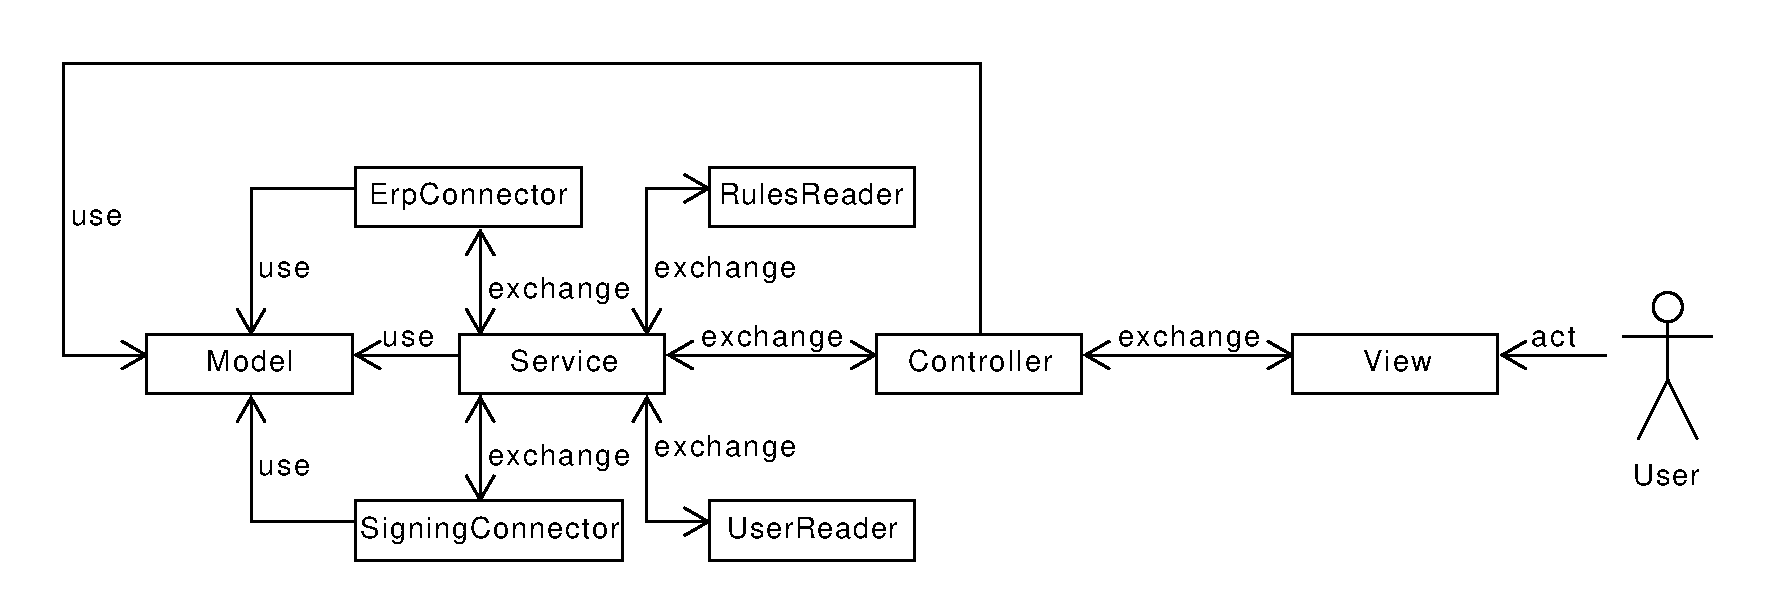
\includegraphics[width=\linewidth]{./design/images/generalCommunication.pdf}
	\caption{General system design}
	\label{fig:generalDesign}
\end{figure}

\subsection*{Enterprise Resource Planning System Connection}
- as variable as possible for ERp systems -> interface specify methods for system

\subsection*{Rule Reader Connection}
- as variable as possible for rule set storage -> interface because every company could have own preferences

\subsection*{Signing Tool Connection}
- as variable as possible for signing tool -> could be changed based on new requirements or company depending: interface

\subsection*{User Reader Connection}
- user management via interface, cause every company could already have existing and to reduce maintenance of data in several dbs 

\section{Used Programming Language and Frameworks}
- why used discussion
- first idea js, but less expiriences not all tools have all functionalities inside Rest api
- Java 8: in company widely used, a lot of experience, time constrains, most SDks available or REST API
- Spring Boot: easy set up, has already a lot of functionalities like security log in, embedded dbs / server, get new experiences, server configurations
- Maven: regulates the dependencies of project, can be build on every machine where maven and java is installed

\begin{table}[h!]
	\begin{tabular}{|l|c|c|} \hline
		Framework/ Tool & Functionality & Usage \\ \hline
		Maven & & \\ \hline
		Spring Boot & & \\ \hline
		Lombock & & \\ \hline
		Mockito & & \\ \hline
		h2 & & \\ \hline
		DocuSign eSign & & \\ \hline
	\end{tabular}
	\centering
	\caption{List used Frameworks}
	\label{tab:frameworks}
\end{table}

\section{Rule Set Request}
Inside the rule set the signing guideline is stored for the system. In general it can be said that there exist four general data sets:
\begin{itemize}
	\item Company positions: \newline
	Inside this data set all the positions of a company are listed, which can be allocated in the company. Each of them has different rights and liabilities.
	\item Document types: \newline
	At a company several different document types exists and they need to be handled differently regarding the signatures. 
	\item Value ranges: \newline
	In a signing guideline several different value ranges are listed. They are inserted in this data set. Each of them has a minimum value and a maximum value.
	\item Signing groups: \newline
	Inside a company several signing groups exists, which consist of different company positions. Each group has combined rights.
\end{itemize}

The rule set is a combination of the previous explained data sets. It defines for each document type and the corresponding value ranges which signing group is allowed to sign the combination. \newline
In the situation a user selects a document for signing, the system needs to analyze based on the document type, the value of the document and the position of the user, if the user is allowed to sign at all and if yes are there other company positions that need to sign along. 

The mathematical presentation of this request is presented in the appendix \ref{mathCode} and the visualization in the appendix \ref{visuRuleset}. ---ToDo: viulization----

\subsection*{Example}
For a better understanding the previous explained theoretical an example is given based on the signing guideline from \gls{cc} presented in table \ref{tab:newSigningGuideline}: \newline
The general data sets:
\begin{itemize}
	\item Company positions: employee; salesman; manager; procurator; chairman
	\item Document types: quotation; \gls{nda}; contract
	\item Value ranges: 0 - 50 000; 50 000,01 - 400 000; 400 000,01 - $\infty$; 0 - $\infty$
	\item Signing groups (extracts): employee only; manager only; salesman with manager; manager with chairman; ....
\end{itemize}

For the rule set example also an extract is selected. In the following the entries are presented:
\begin{enumerate}
	\item Contract; (0 - 50 000); salesman alone
	\item Contract; (0 - 50 000); manager alone
	\item Contract; (0 - 50 000); chairman alone
	\item Contract; (50 000,01 - 400 000); salesman with manager
	\item Contract; (50 000,01 - 400 000); salesman with chairman
	\item Contract; (50 000,01 - 400 000); manager alone
	\item Contract; (50 000,01 - 400 000); chairman alone
	\item Contract; (400 000,01 - $\infty$); salesman with chairman
	\item Contract; (400 000,01 - $\infty$); manager with chairman
	\item Contract; (400 000,01 - $\infty$); chairman alone
\end{enumerate}
	
	\chapter{System Implementation}
	\label{ch:implementation}
	ToDo

\section{Core System}

\section{User Management}
- ldap server, because is used at cc
- mocked, because require more information than currently available at life server
- testing easier
- could be used for customer presentations
- currently no interface directly available due to time issues

\begin{figure}[h!]
	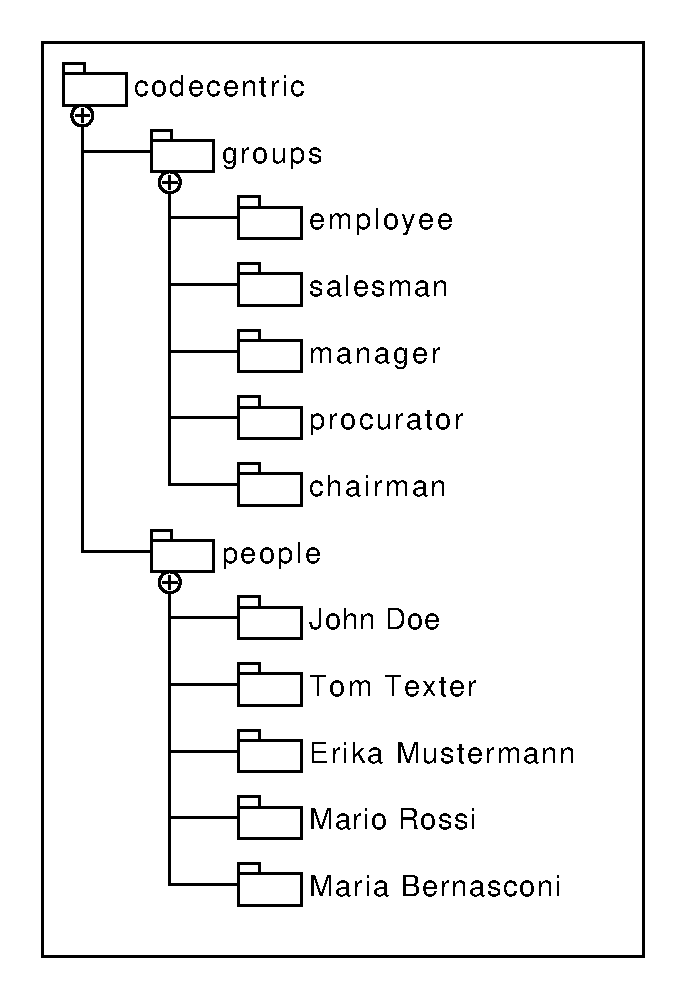
\includegraphics[hight=3cm]{./implementation/images/ldap.pdf}
	\centering
	\caption{Structure of the LDAP Server}
	\label{fig:ldap}
\end{figure}

\section{Enterprise Resource System Connection}
- mocked with very basic functionalities
- only one pdf available for signing -> prototype with 0 logic

\section{Rule Set Implementation}
- started with xml, but later switched to sql because embedded in framework

\begin{figure}[h!]
	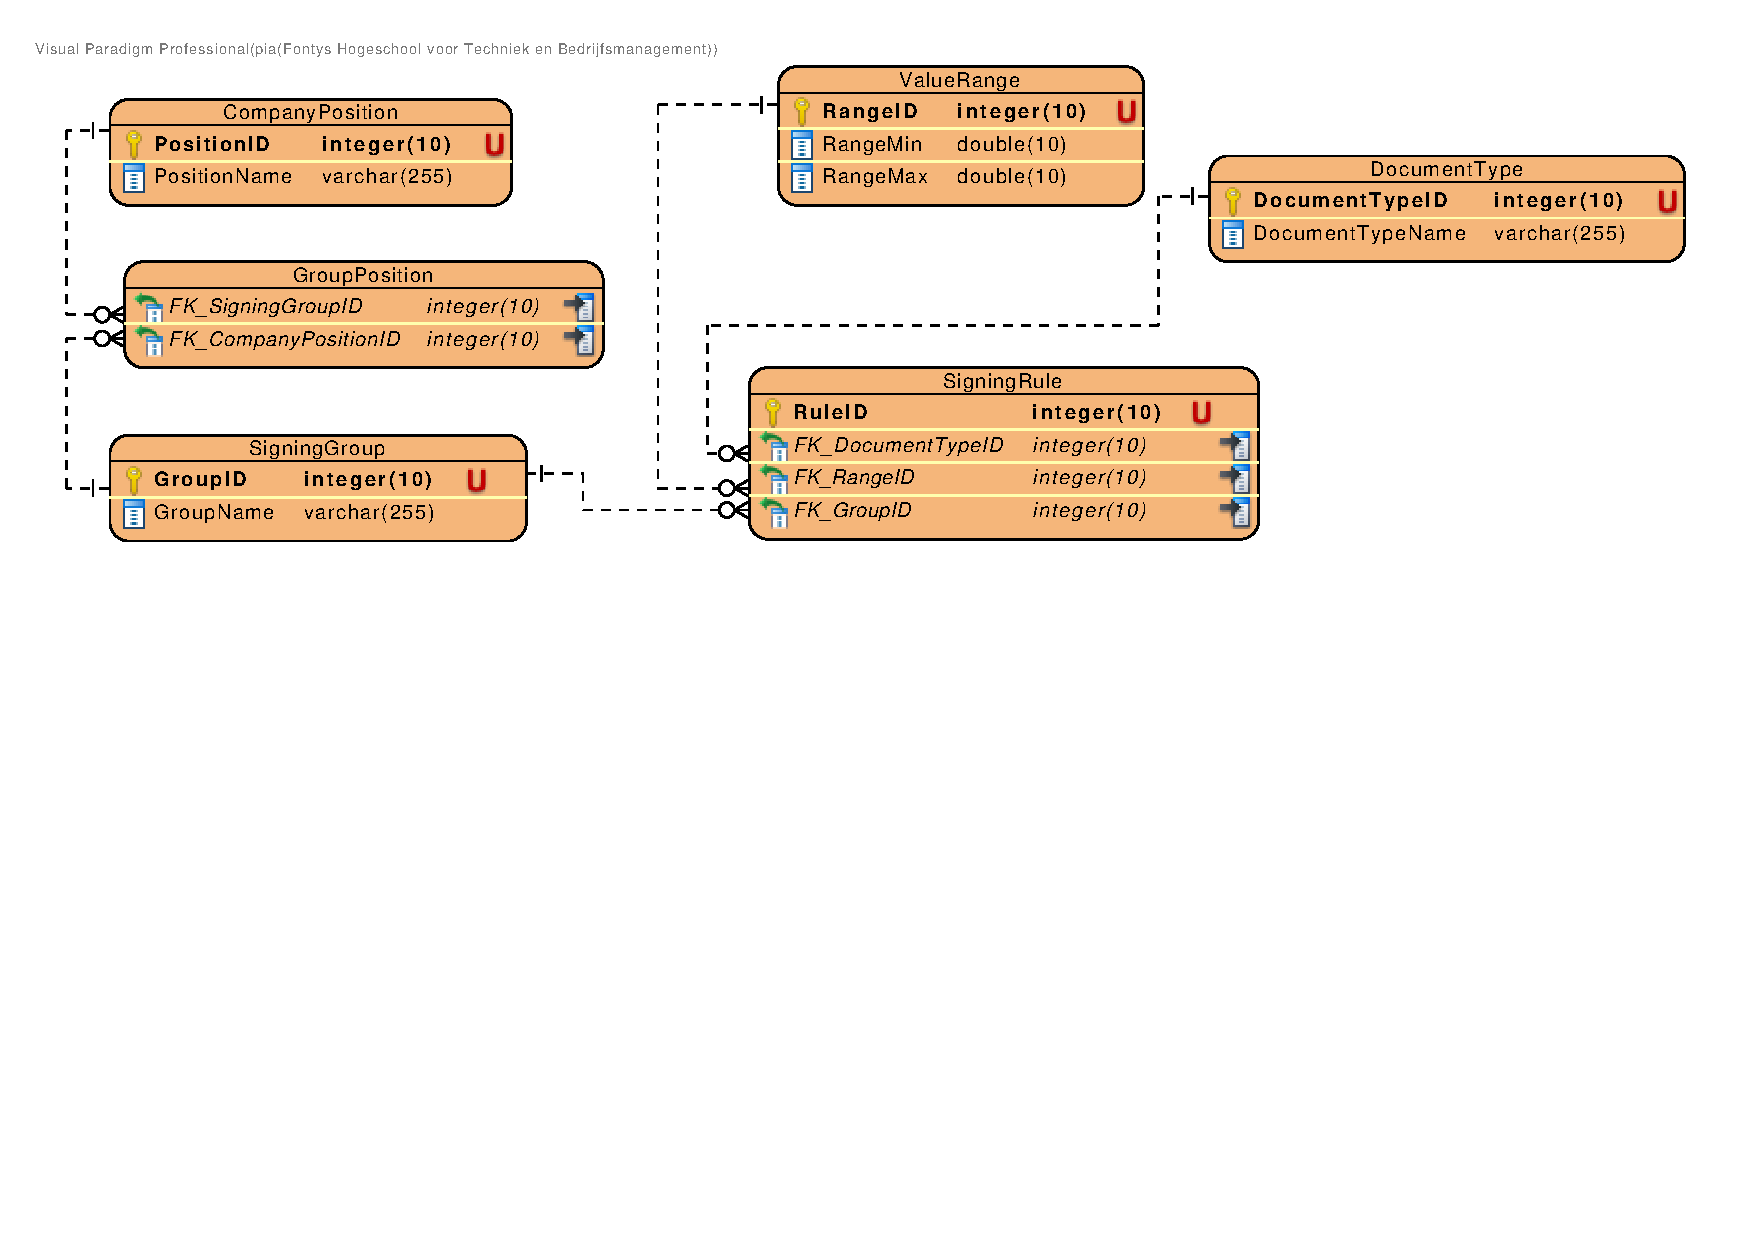
\includegraphics[width=0.6\linewidth]{./implementation/images/db.pdf}
	\centering
	\caption{Entity Relation Diagram of the Rule Set Implementation}
	\label{fig:db}
\end{figure}

\section{Signing System Connection}
- DocuSign API has developer account -> for development and testing 
	
	\chapter{Recommendations}
	\label{ch:advice}
	\section{Advice}
In general need to be said that \glspl{es} are a good alternative for handwriting signatures, especially in \gls{eu} states. The focus is on the type of \gls{es}. The result from the comparison in section \ref{sec:comp} is that the \gls{qes} fits the requirements explained in section \ref{Tab:criteria} best. Also from the legal aspect would it be the best solution, cause of the fact that it is equated to the written signature in the most cases. Even customers with a high demand on legal aspects will be satisfied with that signature, cause of the possibility to track document changes after the signing and the identification of the signers. 
	
	\chapter{Conclusion}
	\label{ch:conclusion}
	At the beginning of the project the plan was to create a \gls{cms} with the possibility to sign documents electronically. 
In the first planning a different customer, \textit{Wacom}, was bet on. That changed, because they did not finish the development of the \gls{sdk} the project should work with. Then it was decided to work for \gls{cc}, because at this moment they do not have a \gls{cms} and they wanted to increase the usage of \gls{es}.

Within their current process they have several problems. The biggest aspects are the amount of manual work that needs to be done with the documents and the issues with the fulfillment of the outdated signing guideline. \newline
To remove the problems, a new process should be created that fulfills the goals of the new signing guideline and reduces manual work and paper usage at \gls{cc}. To introduce and assist the employees to get familiar with the new process, an application should be created, that helps to fulfill the signing guideline with an \gls{es} and coordinates the document storage of signed documents.

Due to the circumstances of high license costs for the signing tool usage and the introduction of a new \gls{erp}, the decision was made to create a prototype, to simulate and check if the application will support the new process. Moreover, it is possible to build the prototype in such a way that it can be combined with any \gls{erp} a company has, as long as it has an \gls{api} to communicate with. It should be as flexible as possible.

During the implementation phase time constrains occurred, that lead to the fact that most functionalities required for simulating the new process are not implemented. It is advisable to pursue development and regularly check the value of the system. But therefore \gls{cc} should wait until they know which new \gls{erp} they get, because there exist a lot of signing tools that are available as plug-in for some \glspl{erp}. It will reduce costs regarding the development and deployment of an own application when they can be connected easily. The only aspect, which needs to be taken into account, is that they may need to make a separate plug-in for checking the signing regulations based on the signing guideline. \newline
In the case no plug-in exists for the new \gls{erp}, the created prototype should be completed and tested for the production at \gls{cc}.

In general it needs to be said, that this bachelor project was not executable as planned due to external circumstances. 
But this could happen with every project that is executed in the working environment of a company.
	
	\printbibliography
	
	\clearpage
	\appendix
	
	\addtocontents{toc}{\protect\setcounter{tocdepth}{1}}
	
	\chapter{Business Sub Process Models of the Old Process}
	\label{bpmnOld}
	\begin{figure}[h]
	\begin{center}
		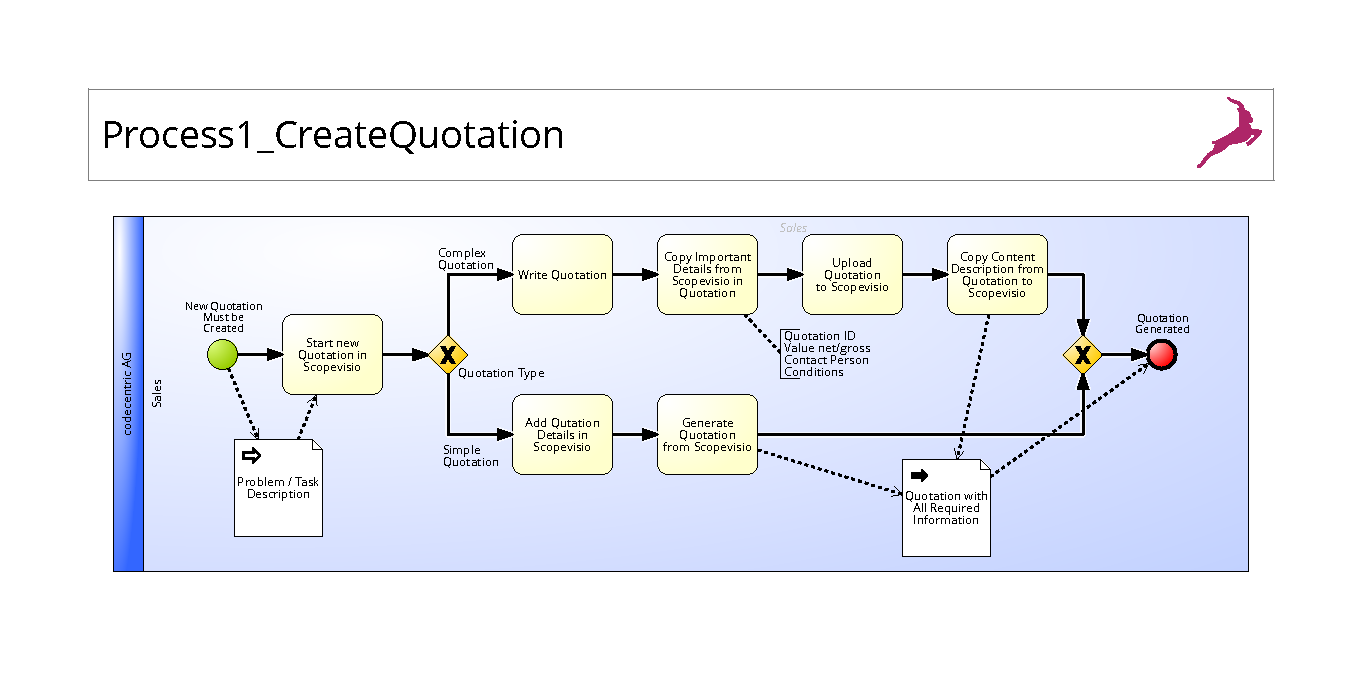
\includegraphics[width=\textheight,angle=90]{./appendix/pbmnOld/0-1_createQuote.pdf}
		\caption{First Old Subprocess - Creation of a Quotation}\label{fig:0-1_sub}
	\end{center}
\end{figure} 

\begin{figure}[h]
	\begin{center}
		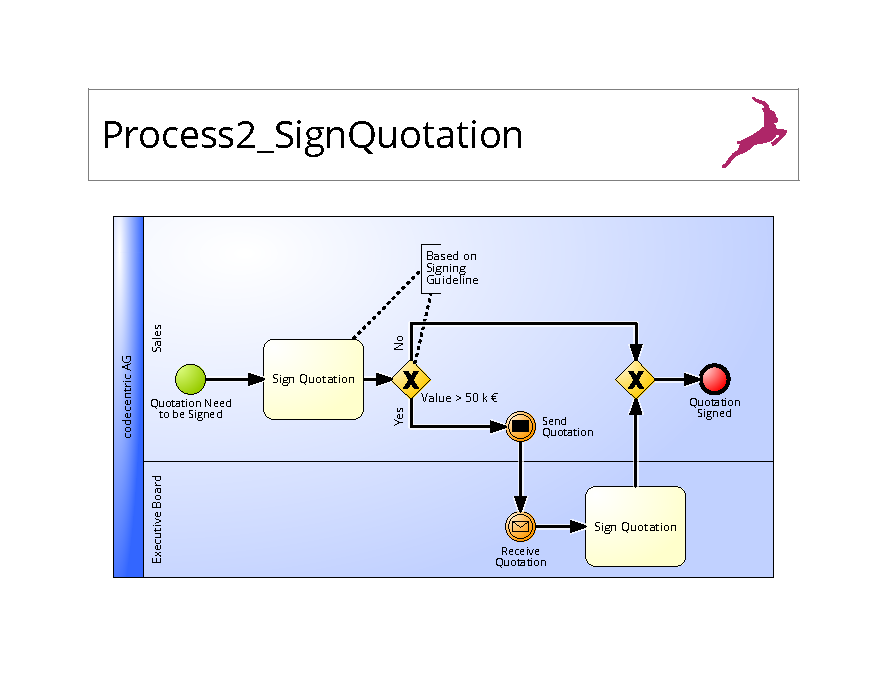
\includegraphics[width=0.8\textwidth]{./appendix/pbmnOld/0-2_signQuote.pdf}
		\caption{Second Old Subprocess - Signing of a Quotation}\label{fig:0-2_sub}
	\end{center}
\end{figure}

\begin{figure}[h]
	\begin{center}
		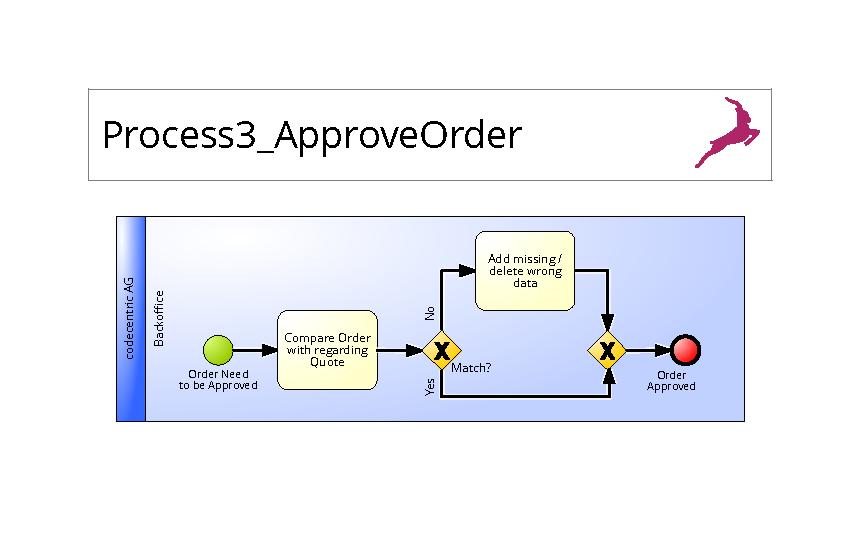
\includegraphics[width=0.8\textwidth]{./appendix/pbmnOld/0-3_approveOrder.pdf}
		\caption{Third Old Subprocess - Approve Order}\label{fig:0-3_sub}
	\end{center}
\end{figure}

\begin{figure}[h]
	\begin{center}
		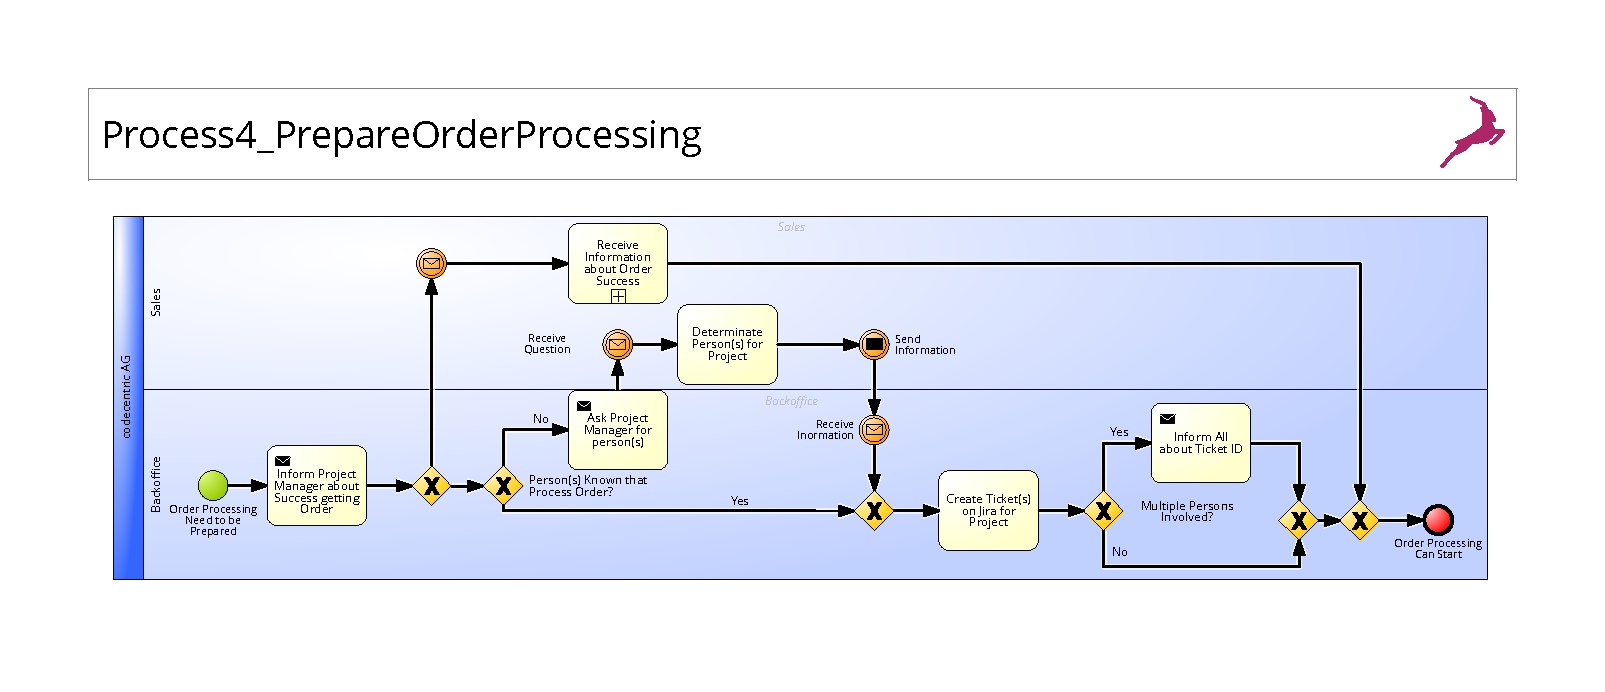
\includegraphics[width=\textheight,angle=90]{./appendix/pbmnOld/0-4_orderProcessing.pdf}
		\caption{Fourth Old Subprocess - Prepare Order Processing}\label{fig:0-4_sub}
	\end{center}
\end{figure}

\begin{figure}[h]
	\begin{center}
		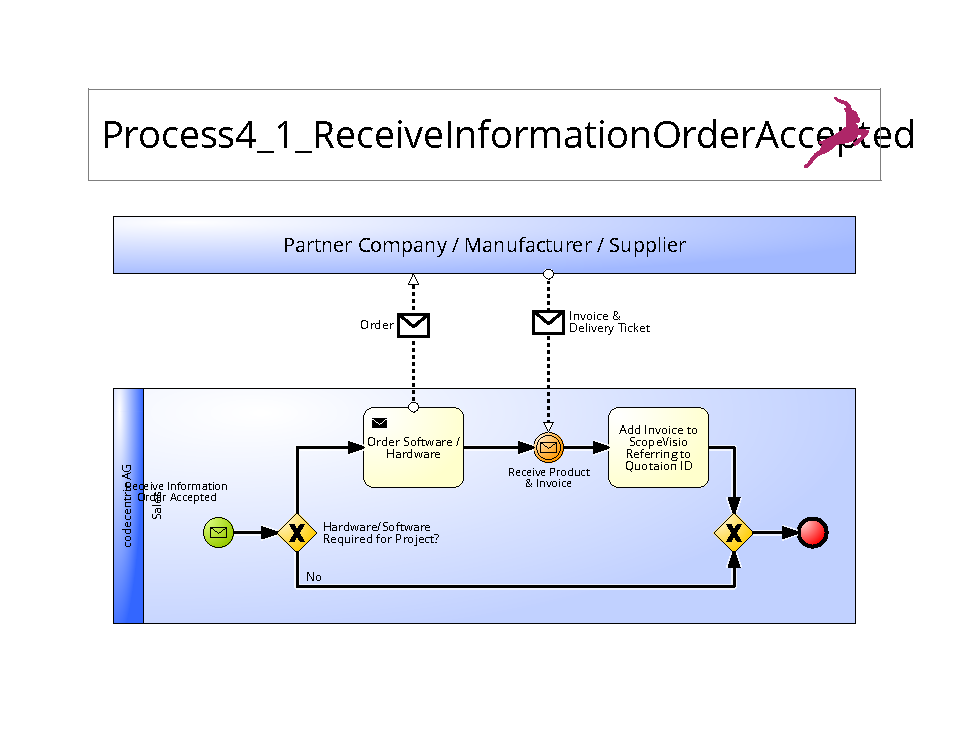
\includegraphics[width=0.8\textwidth]{./appendix/pbmnOld/0-4-1_orderSoftware.pdf}
		\caption{First Old Subsubprocess - Order Needed Hardware and Software}\label{fig:0-4-1_subsub}
	\end{center}
\end{figure}
	
	\chapter{Research about Electronic Signature}
	\label{res:es}
	%This chapter contains the following aspects of a research about \gls{es}, which is part of the second phase of the project: First the scope of the research is described, then the questions which will be answered in this research and how they are answered will be explained. Next the criteria and the weight of them are described to can advice which signature should be used later, followed by presenting the results of the research and a comparison of the different kinds of signatures. Finally, an advice is given. 

\section{Introduction}

At codecentric AG a paperless office should be introduced. That means all contracts and offers possible should be signed and achieved in digitally way. Currently for some contracts a tool is used to sign documents digital, but that should be extended. Also, the achieving is done digital, but in a manual way with scanning of the signed documents and then uploading them to the achieve. Inside this research the topic of \gls{es} is covered, which is part of the paperless office.

This research contains the following aspects of a research: First the scope of the research is described, then the questions which will be answered in this research and how they are answered will be explained. Next the criteria and the weight of them are described to can advice which signature should be used later, followed by presenting the results of the research and a comparison of the different kinds of signatures. Finally, an advice is given.  
\section{Scope}
The scope of this research is to figure out which tool for electronic document signing fits best the requirements given from the company \gls{cc}. Due to the fact that there are many tools available only a selection is done. From the company the tools \textit{HelloSign} and \textit{DocuSign}, solution from partner companies and the solution from the company \textit{Wacom} should be taken into account. Additionally, other tools will be taken into account, but this is only a selection based on an internet research. How this is been done, is explained in the next section.



\section{Questions}

In this research the question will be answered which available tool or technology fits best the requirements of \gls{cc} to sign documents electronically to work more efficient. The  question will be answered through an internet research. Tools will be selected based on the information of different comparison portals and the information provided by the company itself. Furthermore, there will be some testing of the functionalities if possible to prove the usability for \gls{cc}. 

For the testing of the functional requirements like order of singing and the simple usage the preset up is to creation of three test mail addresses and three documents of the format \gls{pdf}, Microsoft word and Open Office writer. The real testing is based on the following steps:
\begin{enumerate}
	\item Register with master mail address to the tool.
	\item Upload the document.
	\item Enter other mail address to sign document.
	\item Select order of signing if possible.
	\item Add fields to sign if needed.
	\item Sign document with master mail address.
	\item Release document for other mail addresses.
	\item Do one of those steps:
	\begin{enumerate}
		\item Try to sign against order.
		\item Try to decline of document signing.
		\item Sign document with unknown account.
		\item Sign document with known accountt. 
	\end{enumerate}
	\item Check current state of the process.
	\item In the case the document is signed by all, check the availability of the document and download it.
\end{enumerate}
\section{Criteria \& Weightings} \label{es:sec:criteria}
Inside this section the different criteria are explained and divided in their weighted categories. The criteria are the following:
\begin{itemize}
	\item Verifiability: \newline
	Importance: 3 \newline
	The signed documents must be legally valid as evidence. In the best case they should have the same legal rights as a document signed with a handwritten signature.
	\item Usability: \newline
	Importance: 2 \newline
	The signing of the documents should be as easy and fast as possible. That means that it should be allowed for cloud services or applications accessible from all possible electronic devices. 
	\item Extra hardware required: \newline
	Importance: 1 \newline
	For some technologies extra hardware is required like a card reader or a component to sign with a pen. That leads to a lot of costs during the fact unknown how many employees need to have such hardware.
\end{itemize} 

The table \ref{ES:Tab:criteria} displays the different categories for each criterion and shows their weighting. The best weighting is (+ +) and the worst is (- -). 

\begin{table}[h]
	\centering
	\begin{tabular}{|c|c|c|} \hline
		\rowcolor{Gray}Criterion  & Category & Weighting \\ \hline
		\multirow{4}{*}{Verifiability} & No & - - \\ \cline{2-3}
									   & Yes & o \\ \cline{2-3}
									   & With tracking of documents changes & + \\ \cline{2-3}
									   & Equal to handwritten signature & + + \\ \cline{1-3}
		\multirow{3}{*}{Usability} & Only PC & - - \\ \cline{2-3}
		                           & Only devices with touch recognition & - \\ \cline{2-3}
								   & All devices & + + \\ \cline{1-3}
		\multirow{3}{*}{Extra hardware required} & Yes & - -\\ \cline{2-3}
												& Possible & o \\ \cline{2-3}
												& No & + +  \\ \cline{1-3}
	\end{tabular}
	\caption{Categories and their weighting}
	\label{ES:Tab:criteria}
\end{table}
\section{Result}
In this section different tools will be described, their test result presented and the general information of them summarized.

\subsection{Wacom sign pro PDF}
This tool is provided by the company Wacom, which is the customer previously thought for the bachelor project. At the moment there is an \gls{app} available, that signs documents with a \gls{bs} \parencite{wacom2018pdf}. Currently Wacom develops an \gls{sdk} based on the \gls{app}, therefore is no testing possible. The information presented in table \ref{tab:wacom} are from the internet and a product presentation from first March 2018 at the Wacom site in Düsseldorf. 
\begin{table}[h]
	\begin{tabular}{|p{4cm}|p{10cm}|} \hline
		Criterion & Fulfillment \\ \hline
		Usage without license & At the moment not clear. The \gls{app} currently has a free version, but with limited usage.\\ \hline
		Devices independent & The usage of this technology requires hardware at the moment. Therefore, several options exist. Either you have a smart phone with a pen, an iOS phone, a Windows computer with touch recognition or a Windows computer with additional hardware.\\ \hline
		Integration possible & This year a new \gls{sdk} will be published that allows the integration with existing tools. \\ \hline
		Certified & The software uses the \gls{bs} and \gls{aes}. Currently there is no defined status by the government for the \gls{bs}. But in combination with the \gls{aes} it has a legal status. \\ \hline
		Easy usage & Select field(s) to enter data and sign with the pen, press button to agree and then enter mail to sharing. It is not described if a company stamp could be inserted.\\ \hline
		Costs & Unclear, due to the fact that the \gls{sdk} is not published and no pricing is published.\\ \hline
		Accepted documents & \Gls{pdf}\\ \hline
		Amount of accounts & At the moment also unclear due to the fact that the usage requirements are not published. The \gls{app} currently allows more than 5000 in one environment. \\ \hline
	\end{tabular}
	\caption{Summary Wacom sign pro PDF}
	\label{tab:wacom}
\end{table}

\subsection{DocuSign}
This tool is already in usage at \gls{cc}, but not always and with a lot of manual actions and missing things like the company stamp. During the testing a lot of functionalities were figured out. The test protocol is placed in the appendix \ref{sec:docusign}. The table \ref{tab:docusign} below will give a short summary about the test result and other aspects figured out during the research.

\begin{table}[h]
	\begin{tabular}{|p{4cm}|p{10cm}|} \hline
		Criterion & Fulfillment \\ \hline
		Usage without license & Yes, just need to add some information required from the person request the signing like name and mail address for signing. In the case of uploading and managing the documents an account is required.\\ \hline
		Devices independent & Online available, also a \gls{app} is accessible for all \gls{os} of smartphones \parencite{docusign2018mobile}. \\ \hline
		Integration possible & A \gls{sdk} available within the \grqq Business Flex\grqq packet of the provider. Also an integration is possible with Google Drive, but therefore the Google Drive cloud need to be connected to DocuSign \parencite{docusign2018integration,docusign2018formats}. \\ \hline
		Certified & DocuSign satisfies the standards of the \gls{eidas} and more security standards \parencite{docusign2018certificates,docusign2018legal}. \\ \hline
		Easy usage & The fields need to be set manual, it need to be checked if it possible to customize it. Furthermore it is possible to track activities, assign signer, add the company stamp, transfer the signing responsibility, decline the signing and to sign the document manual and scan it then. \\ \hline
		Costs & The provider of DocuSign offers different plans. \Gls{cc} needs at least the \textit{Business Pro} Plan for one user, which costs 480\$ per year, and the \textit{intermediate API} plan with 3420\$ per year. But due to the fact, that there will  e more than one user, the enterprise offerings should be requested. \parencite{docusign2018api,docusign2018user} \\ \hline
		Accepted documents & PDF \& Microsoft Word accepted, Open Office Writer is not accepted. Moreover, the maximum accepted size of a document is 25 \gls{mb}. \parencite{docusign2018formats} \\ \hline
		Amount of accounts & Depending on the license ordered.\\ \hline
	\end{tabular}
	\caption{Summary DocuSign}
	\label{tab:docusign}
\end{table}

\subsection{HelloSign}
The online tool HelloSign is used at the subsidiary company Istana of \gls{cc}. Therefore, it should also taken into account. Not all functionalities could be tested through the fact that for the business version data were requested, the tester was not allowed to give. The result of the test is documented in appendix \ref{sec:hellosign} and a summary of it together with additional information collected from an online research is given in table \ref{tab:hellosign}.
\begin{table}[h]
	\begin{tabular}{|p{4cm}|p{10cm}|} \hline
		Criterion & Fulfillment \\ \hline
		Usage without license & Signing without account possible, but the signed documents could not be viewed online and uploaded if no account exists. It will be send within a mail. Moreover, there is the fact that the free version only allows to send three documents per month. This leads to the result, that a higher version is required \parencite{hellosign2018price}. \\ \hline
		Devices independent & The tool is online available. Furthermore, exists an \gls{app} for Android and iOS, but it has not the same functionalities as the online platform.  \parencite{hellosign2018legal} \\ \hline
		Integration possible & HelloSign has an \gls{api} with different version provided, included there are several functionalities. Moreover, integration exists for Google services like Google Suite and for several other business applications e.g. HubSpot CRM, which used at \gls{cc}. Additionally third party integrations are possible with Zapier, a tool for modeling business processes. \parencite{hellosign2018integration,hellosign2018api} \\ \hline
		Certified & The tool fulfills the requirements of the \gls{eidas} regulations of the \gls{eu} and can be used in the \gls{usa} \parencite{hellosign2018legal} \\ \hline
		Easy usage & It is simple to upload a document and sign it, due to the fact that there is intuitive handling. Not all functionalities like branding and company stamp could be tested, because of the non usable test version of higher plans. The fields required for signing need to be set manual and there is not that much choice of fields. In the case the \gls{app} is used, only the creation of a signing process could be done. \\ \hline
		Costs & For the usage at \gls{cc} two different licenses are required. First the \gls{api} license where at least the version API Gold is need which costs 449\$ per month. The second license is the user license. Therefore the User Business version is required at least with five senders. It costs 40\$ per month. But due to the fact, that more senders are needed the Enterprise version is advisable. Yet the price is not given in the internet\parencite{hellosign2018price,hellosign2018api} .\\ \hline
		Accepted documents & HelloSign accepts several documents format. In the test the formats \gls{pdf}, Microsoft Word and Open Office Writer was accepted. The maximal amount of a pages a document is 500 pages or a file size of 40th \gls{mb} \parencite{hellosign2018documents}. \\ \hline
		Amount of accounts & Inside the business version of HelloSign 5 senders/accounts are involved, for more accounts the provider need to be requested \parencite{hellosign2018price}. \\ \hline
	\end{tabular}
	\caption{Summary HelloSign}
	\label{tab:hellosign}
\end{table}

\subsection{SignDoc}
This tool is provided by Kofax, a partner of \gls{cc}.

\begin{table}[h]
	\begin{tabular}{|p{4cm}|p{10cm}|} \hline
		Criterion & Fulfillment \\ \hline
		Usage without license & \\ \hline
		Devices independent & \\ \hline
		Integration possible & \\ \hline
		Certified & \\ \hline
		Easy usage & \\ \hline
		Costs & \\ \hline
		Accepted documents & \\ \hline
		Amount of accounts & \\ \hline
	\end{tabular}
	\caption{Summary SignDoc}
	\label{tab:signdoc}
\end{table}

\subsection{Adobe Sign}

\begin{table}[h]
	\begin{tabular}{|p{4cm}|p{10cm}|} \hline
		Criterion & Fulfillment \\ \hline
		Usage without license & yes, but for starting license required\\ \hline
		Devices independent & web, app iOS and Android (require certain os version) \\ \hline
		Integration possible & A lot of integration with tools possible, api available \parencite{adobesign2018integration,adobesign2018info} \\ \hline
		Certified & eIdas \parencite{adobesign2018legal} \\ \hline
		Easy usage & \\ \hline
		Costs & Enterprise plan required, but no price published online \parencite{adobesign2018costs} \\ \hline
		Accepted documents & PDF, Microsoft Word \parencite{adobesign2018info} \\ \hline
		Amount of accounts & Unknown \\ \hline
	\end{tabular}
	\caption{Summary Adobe Sign}
	\label{tab:adobesign}
\end{table}

\subsection{SignNow}

\begin{table}[h]
	\begin{tabular}{|p{4cm}|p{10cm}|} \hline
		Criterion & Fulfillment \\ \hline
		Usage without license & \\ \hline
		Devices independent & \\ \hline
		Integration possible & \\ \hline
		Certified & \\ \hline
		Easy usage & \\ \hline
		Costs & \\ \hline
		Accepted documents & \\ \hline
		Amount of accounts & \\ \hline
	\end{tabular}
	\caption{Summary SignNow}
	\label{tab:signnow}
\end{table}

\subsection{RightSignature}

\begin{table}[h]
	\begin{tabular}{|p{4cm}|p{10cm}|} \hline
		Criterion & Fulfillment \\ \hline
		Usage without license & \\ \hline
		Devices independent & \\ \hline
		Integration possible & \\ \hline
		Certified & \\ \hline
		Easy usage & \\ \hline
		Costs & \\ \hline
		Accepted documents & \\ \hline
		Amount of accounts & \\ \hline
	\end{tabular}
	\caption{Summary RightSignature}
	\label{tab:rightsignature}
\end{table}

\subsection{eSign Live}

\begin{table}[h]
	\begin{tabular}{|p{4cm}|p{10cm}|} \hline
		Criterion & Fulfillment \\ \hline
		Usage without license & \\ \hline
		Devices independent & \\ \hline
		Integration possible & \\ \hline
		Certified & \\ \hline
		Easy usage & \\ \hline
		Costs & \\ \hline
		Accepted documents & \\ \hline
		Amount of accounts & \\ \hline
	\end{tabular}
	\caption{Summary eSign Live}
	\label{tab:esign}
\end{table}

\subsection{PandaDoc}

\begin{table}[h]
	\begin{tabular}{|p{4cm}|p{10cm}|} \hline
		Criterion & Fulfillment \\ \hline
		Usage without license & \\ \hline
		Devices independent & \\ \hline
		Integration possible & \\ \hline
		Certified & \\ \hline
		Easy usage & \\ \hline
		Costs & \\ \hline
		Accepted documents & \\ \hline
		Amount of accounts & \\ \hline
	\end{tabular}
	\caption{Summary PandaDoc}
	\label{tab:pandadoc}
\end{table}

\subsection{eSignAnyWhere}

\section{Comparison} \label{sec:comp}

\section{Advice}
In general need to be said that \glspl{es} are a good alternative for handwriting signatures, especially in \gls{eu} states. The focus is on the type of \gls{es}. The result from the comparison in section \ref{sec:comp} is that the \gls{qes} fits the requirements explained in section \ref{Tab:criteria} best. Also from the legal aspect would it be the best solution, cause of the fact that it is equated to the written signature in the most cases. Even customers with a high demand on legal aspects will be satisfied with that signature, cause of the possibility to track document changes after the signing and the identification of the signers. 
	
	\chapter{Research about Signing Tool}
	\label{res:tool}
	\section{Introduction}

At codecentric AG a paperless office should be introduced. That means all contracts and offers possible should be signed and achieved in digitally way. Currently for some contracts a tool is used to sign documents digital, but that should be extended. Also, the achieving is done digital, but in a manual way with scanning of the signed documents and then uploading them to the achieve. Inside this research the topic of \gls{es} is covered, which is part of the paperless office.

This research contains the following aspects of a research: First the scope of the research is described, then the questions which will be answered in this research and how they are answered will be explained. Next the criteria and the weight of them are described to can advice which signature should be used later, followed by presenting the results of the research and a comparison of the different kinds of signatures. Finally, an advice is given.  
\section{Scope}
The scope of this research is to figure out which tool for electronic document signing fits best the requirements given from the company \gls{cc}. Due to the fact that there are many tools available only a selection is done. From the company the tools \textit{HelloSign} and \textit{DocuSign}, solution from partner companies and the solution from the company \textit{Wacom} should be taken into account. Additionally, other tools will be taken into account, but this is only a selection based on an internet research. How this is been done, is explained in the next section.



\section{Questions}

In this research the question will be answered which available tool or technology fits best the requirements of \gls{cc} to sign documents electronically to work more efficient. The  question will be answered through an internet research. Tools will be selected based on the information of different comparison portals and the information provided by the company itself. Furthermore, there will be some testing of the functionalities if possible to prove the usability for \gls{cc}. 

For the testing of the functional requirements like order of singing and the simple usage the preset up is to creation of three test mail addresses and three documents of the format \gls{pdf}, Microsoft word and Open Office writer. The real testing is based on the following steps:
\begin{enumerate}
	\item Register with master mail address to the tool.
	\item Upload the document.
	\item Enter other mail address to sign document.
	\item Select order of signing if possible.
	\item Add fields to sign if needed.
	\item Sign document with master mail address.
	\item Release document for other mail addresses.
	\item Do one of those steps:
	\begin{enumerate}
		\item Try to sign against order.
		\item Try to decline of document signing.
		\item Sign document with unknown account.
		\item Sign document with known accountt. 
	\end{enumerate}
	\item Check current state of the process.
	\item In the case the document is signed by all, check the availability of the document and download it.
\end{enumerate}
\section{Criteria \& Weightings} \label{tool:sec:criteria}
Inside this section the different criteria are explained and divided in their
weighted categories. The criteria are the following:
\begin{itemize}
	\item Integration \newline
	Weight: 8 \newline
		The most important criterion is the integration, because the tool should be interact with the \gls{erp} and the Google Suite used by \gls{cc}. In the best case all the tools can be used in one system. This means they are in such a way integrated with each other, that the end user do not need to switch the applications. \newline
		This criterion is a knockout criterion. In the case it is not fulfilled the tool will be automatically ignored for the process realization. 
	\item Device independent \newline
	Weight: 7 \newline
	Due to the fact that all employees of \gls{cc} have different \gls{os} for their computer and smart phones, should be the tool hardware independent. Furthermore, it is stated that the employees and execution board is not always at the buildings of the company available, doing home office or working by the customers. This leads to the preference of having \gls{app} for the tool, so that the employees of \gls{cc} can sign the documents everywhere they are independent of their device available.\newline
	This criterion is a knockout criterion. In the case it is not fulfilled the tool will be automatically ignored for the process realization. 
	\item Usability \newline
	Weight: 6 \newline
	Another requirement is the usability. For the reason that several employees should use the tool, it need to be simple to use. There should be no long learning time and the handling need be intuitive or at least the tool should provide information about buttons or next steps. In the best case the tool has a lot of automated processes, so that the user do not care about what to add where and with which information.
	\item Costs \newline
	Weight: 5 \newline
	It is important to have the costs in focus. If they are too high the cost-benefit ratio will be negative and the effect of the new process for \gls{cc} is non existing. The areas pricing model, access to functionalities and amount of accounts fall into this category. For this research price information for 2.400 documents and 80 users should be collected and then calculate this price for one document to get information about the price per document. The classification should be done based on the average of all tools taken into account.
	\item Accepted file formats \newline
	Weight: 4 \newline
	\Gls{cc} uses in general three different file formats for their documents. It should with the tool possible to use them in the future with the tool to sign the documents without converting them into another format.
	\item Operating mode \newline
	Weight: 3 \newline
	Another criterion is the operating mode. That means runs the tool as \gls{saas} or \gls{op}, need \gls{cc} provide its own server and need to care about its security and backup or does the provider of the tool offers this within his plan. This influence also the costs of the tool.
	\item Additional security \newline
	Weight: 2 \newline
	To be sure that the correct person use the service and to increase the security, \gls{cc} uses the Two-Factor authentication for most systems and tools they use. This should be also available for the signature tool.
	\item Legal aspects \newline
	Weight: 1 \newline
	The tool should satisfy certain legal standards, so that \gls{cc} could be use the signing as evidence. This is also important in respect to further use cases for the tool at \gls{cc}, where a higher standard exist than for quotations.
\end{itemize}

The table \ref{tool:tab:resTcateg} displays the different categories for each criterion and shows
their weighting. The best weighting is (+ +) and the worst is (- -). 

%\begin{table}[h!]
	\begin{longtable}{|p{4cm}|p{9cm}|p{1.5cm}|} \hline
		\rowcolor{Gray}Criterion & Category & Weighting \\ \hline
		\multirow{6}{*}{Integration} & No & - - \\ \cline{2-3}
									& Tools for workflow building & o \\ \cline{2-3}
									& Predefined integrations for some tools at \gls{cc} exists already & o \\ \cline{2-3}
									& \Gls{api} and/or \gls{sdk} & + \\ \cline{2-3}
									& \Gls{api} and/or \gls{sdk} \& predefined integrations for some tools that are already in usage & + + \\ \cline{2-3}
									& Predefined integrations for all tools used at \gls{cc} & + + \\ \hline 
		\multirow{8}{*}{Device independent} & Additional hardware required & - - \\ \cline{2-3}
											& Only for certain \gls{os} for Desktop & - - \\ \cline{2-3}
											& Only for certain \gls{os} for smart phone & - - \\ \cline{2-3} 
											& Only for Desktop & - \\ \cline{2-3}
											& Only for smart phone & o \\ \cline{2-3}
											& Only for programmed devices & o \\ \cline{2-3}
											& Only web application & + \\ \cline{2-3}
											& With web application and for all \gls{os} of smart phone and Desktop & + + \\ \hline
		\multirow{5}{*}{Usability} & A lot of actions to set required fields \& activate sharing & - - \\ \cline{2-3}
								    & A few actions to set required fields \& activate sharing & o \\ \cline{2-3}
									& A few actions to set required fields \& activate sharing \& company stamp can be recorded & + \\ \cline{2-3}
									& Recognize where to set fields & + \\ \cline{2-3}
									& Recognize where to set fields \& company stamp can be recorded & + + \\ \hline
		\multirow{5}{*}{Costs}  & $ \textgreater +25\% \varnothing $ & - - \\ \cline{2-3}
								& $ \textgreater \varnothing \& \leq +25\% \varnothing $ & - \\ \cline{2-3}
								& $ \textgreater -25\% \varnothing \& \leq \varnothing  $ & o \\ \cline{2-3}
								& $ \textgreater -50\% \varnothing \& \leq -25\% \varnothing $ & + \\ \cline{2-3}
								& $ \leq -50\% \varnothing $ & + + \\ \hline
		\multirow{4}{*}{Accepted file formats} & Special type & - - \\ \cline{2-3}
												& \Gls{PDF} & o \\ \cline{2-3}
												& \Gls{PDF} \& Microsoft Word (doc, docx) & + \\ \cline{2-3}
												& \Gls{PDF}, Microsoft Word \& Open Office Writer(odt) & + + \\ \hline
		\multirow{2}{*}{Operating mode} & \gls{op} & o \\ \cline{2-3}
										 & \gls{saas} & + + \\ \hline
		\multirow{6}{*}{Additional security} & None & - - \\ \cline{2-3}
											& Question and Answer & o \\ \cline{2-3} 
											& Online identity & o \\ \cline{2-3}
											& Authentication with mobile phone & + \\ \cline{2-3}
											& Authentication with video, personal ID or similar & + + \\ \cline{2-3}
											& Certification & + + \\ \hline
		\multirow{6}{*}{Legal aspects} & No & - - \\ \cline{2-3}
										& \gls{eidas} fulfilled with \gls{ses} & - \\ \cline{2-3}
										& \gls{eidas} \& \glossary{gdpr} fulfilled with \gls{ses} & o \\ \cline{2-3}
										& \gls{eidas} \& \glossary{gdpr} fulfilled with \gls{aes} or \gls{qes} & + \\ \cline{2-3}
										& \gls{eidas} \& \glossary{gdpr} fulfilled with \gls{aes} or \gls{qes} \& global accepted & + + \\ \hline
	\caption{Categories and their weighings}
	\label{tool:tab:resTcateg}
	\end{longtable}
%	\caption{Categories and their weighings}
%	\label{tab:resTcateg}
%\end{table}
%\newpage
\section{Result}
In this section different tools will be described, their test result presented and the general information of them summarized.

\subsection{Wacom sign pro PDF}
This tool is provided by the company Wacom, which is the customer previously thought for the bachelor project. At the moment there is an \gls{app} available, that signs documents with a \gls{bs} \parencite{wacom2018pdf}. Currently Wacom develops an \gls{sdk} based on the \gls{app}, therefore is no testing possible. The information presented in table \ref{tab:wacom} are from the internet and a product presentation from first March 2018 at the Wacom site in Düsseldorf. 
\begin{table}[h]
	\begin{tabular}{|p{4cm}|p{10cm}|} \hline
		Criterion & Fulfillment \\ \hline
		Usage without license & At the moment not clear. The \gls{app} currently has a free version, but with limited usage.\\ \hline
		Devices independent & The usage of this technology requires hardware at the moment. Therefore, several options exist. Either you have a smart phone with a pen, an iOS phone, a Windows computer with touch recognition or a Windows computer with additional hardware.\\ \hline
		Integration possible & This year a new \gls{sdk} will be published that allows the integration with existing tools. \\ \hline
		Certified & The software uses the \gls{bs} and \gls{aes}. Currently there is no defined status by the government for the \gls{bs}. But in combination with the \gls{aes} it has a legal status. \\ \hline
		Easy usage & Select field(s) to enter data and sign with the pen, press button to agree and then enter mail to sharing. It is not described if a company stamp could be inserted.\\ \hline
		Costs & Unclear, due to the fact that the \gls{sdk} is not published and no pricing is published.\\ \hline
		Accepted documents & \Gls{pdf}\\ \hline
		Amount of accounts & At the moment also unclear due to the fact that the usage requirements are not published. The \gls{app} currently allows more than 5000 in one environment. \\ \hline
	\end{tabular}
	\caption{Summary Wacom sign pro PDF}
	\label{tab:wacom}
\end{table}

\subsection{DocuSign}
This tool is already in usage at \gls{cc}, but not always and with a lot of manual actions and missing things like the company stamp. During the testing a lot of functionalities were figured out. The test protocol is placed in the appendix \ref{sec:docusign}. The table \ref{tab:docusign} below will give a short summary about the test result and other aspects figured out during the research.

\begin{table}[h]
	\begin{tabular}{|p{4cm}|p{10cm}|} \hline
		Criterion & Fulfillment \\ \hline
		Usage without license & Yes, just need to add some information required from the person request the signing like name and mail address for signing. In the case of uploading and managing the documents an account is required.\\ \hline
		Devices independent & Online available, also a \gls{app} is accessible for all \gls{os} of smartphones \parencite{docusign2018mobile}. \\ \hline
		Integration possible & A \gls{sdk} available within the \grqq Business Flex\grqq packet of the provider. Also an integration is possible with Google Drive, but therefore the Google Drive cloud need to be connected to DocuSign \parencite{docusign2018integration,docusign2018formats}. \\ \hline
		Certified & DocuSign satisfies the standards of the \gls{eidas} and more security standards \parencite{docusign2018certificates,docusign2018legal}. \\ \hline
		Easy usage & The fields need to be set manual, it need to be checked if it possible to customize it. Furthermore it is possible to track activities, assign signer, add the company stamp, transfer the signing responsibility, decline the signing and to sign the document manual and scan it then. \\ \hline
		Costs & The provider of DocuSign offers different plans. \Gls{cc} needs at least the \textit{Business Pro} Plan for one user, which costs 480\$ per year, and the \textit{intermediate API} plan with 3420\$ per year. But due to the fact, that there will  e more than one user, the enterprise offerings should be requested. \parencite{docusign2018api,docusign2018user} \\ \hline
		Accepted documents & PDF \& Microsoft Word accepted, Open Office Writer is not accepted. Moreover, the maximum accepted size of a document is 25 \gls{mb}. \parencite{docusign2018formats} \\ \hline
		Amount of accounts & Depending on the license ordered.\\ \hline
	\end{tabular}
	\caption{Summary DocuSign}
	\label{tab:docusign}
\end{table}

\subsection{HelloSign}
The online tool HelloSign is used at the subsidiary company Istana of \gls{cc}. Therefore, it should also taken into account. Not all functionalities could be tested through the fact that for the business version data were requested, the tester was not allowed to give. The result of the test is documented in appendix \ref{sec:hellosign} and a summary of it together with additional information collected from an online research is given in table \ref{tab:hellosign}.
\begin{table}[h]
	\begin{tabular}{|p{4cm}|p{10cm}|} \hline
		Criterion & Fulfillment \\ \hline
		Usage without license & Signing without account possible, but the signed documents could not be viewed online and uploaded if no account exists. It will be send within a mail. Moreover, there is the fact that the free version only allows to send three documents per month. This leads to the result, that a higher version is required \parencite{hellosign2018price}. \\ \hline
		Devices independent & The tool is online available. Furthermore, exists an \gls{app} for Android and iOS, but it has not the same functionalities as the online platform.  \parencite{hellosign2018legal} \\ \hline
		Integration possible & HelloSign has an \gls{api} with different version provided, included there are several functionalities. Moreover, integration exists for Google services like Google Suite and for several other business applications e.g. HubSpot CRM, which used at \gls{cc}. Additionally third party integrations are possible with Zapier, a tool for modeling business processes. \parencite{hellosign2018integration,hellosign2018api} \\ \hline
		Certified & The tool fulfills the requirements of the \gls{eidas} regulations of the \gls{eu} and can be used in the \gls{usa} \parencite{hellosign2018legal} \\ \hline
		Easy usage & It is simple to upload a document and sign it, due to the fact that there is intuitive handling. Not all functionalities like branding and company stamp could be tested, because of the non usable test version of higher plans. The fields required for signing need to be set manual and there is not that much choice of fields. In the case the \gls{app} is used, only the creation of a signing process could be done. \\ \hline
		Costs & For the usage at \gls{cc} two different licenses are required. First the \gls{api} license where at least the version API Gold is need which costs 449\$ per month. The second license is the user license. Therefore the User Business version is required at least with five senders. It costs 40\$ per month. But due to the fact, that more senders are needed the Enterprise version is advisable. Yet the price is not given in the internet\parencite{hellosign2018price,hellosign2018api} .\\ \hline
		Accepted documents & HelloSign accepts several documents format. In the test the formats \gls{pdf}, Microsoft Word and Open Office Writer was accepted. The maximal amount of a pages a document is 500 pages or a file size of 40th \gls{mb} \parencite{hellosign2018documents}. \\ \hline
		Amount of accounts & Inside the business version of HelloSign 5 senders/accounts are involved, for more accounts the provider need to be requested \parencite{hellosign2018price}. \\ \hline
	\end{tabular}
	\caption{Summary HelloSign}
	\label{tab:hellosign}
\end{table}

\subsection{SignDoc}
This tool is provided by Kofax, a partner of \gls{cc}.

\begin{table}[h]
	\begin{tabular}{|p{4cm}|p{10cm}|} \hline
		Criterion & Fulfillment \\ \hline
		Usage without license & \\ \hline
		Devices independent & \\ \hline
		Integration possible & \\ \hline
		Certified & \\ \hline
		Easy usage & \\ \hline
		Costs & \\ \hline
		Accepted documents & \\ \hline
		Amount of accounts & \\ \hline
	\end{tabular}
	\caption{Summary SignDoc}
	\label{tab:signdoc}
\end{table}

\subsection{Adobe Sign}

\begin{table}[h]
	\begin{tabular}{|p{4cm}|p{10cm}|} \hline
		Criterion & Fulfillment \\ \hline
		Usage without license & yes, but for starting license required\\ \hline
		Devices independent & web, app iOS and Android (require certain os version) \\ \hline
		Integration possible & A lot of integration with tools possible, api available \parencite{adobesign2018integration,adobesign2018info} \\ \hline
		Certified & eIdas \parencite{adobesign2018legal} \\ \hline
		Easy usage & \\ \hline
		Costs & Enterprise plan required, but no price published online \parencite{adobesign2018costs} \\ \hline
		Accepted documents & PDF, Microsoft Word \parencite{adobesign2018info} \\ \hline
		Amount of accounts & Unknown \\ \hline
	\end{tabular}
	\caption{Summary Adobe Sign}
	\label{tab:adobesign}
\end{table}

\subsection{SignNow}

\begin{table}[h]
	\begin{tabular}{|p{4cm}|p{10cm}|} \hline
		Criterion & Fulfillment \\ \hline
		Usage without license & \\ \hline
		Devices independent & \\ \hline
		Integration possible & \\ \hline
		Certified & \\ \hline
		Easy usage & \\ \hline
		Costs & \\ \hline
		Accepted documents & \\ \hline
		Amount of accounts & \\ \hline
	\end{tabular}
	\caption{Summary SignNow}
	\label{tab:signnow}
\end{table}

\subsection{RightSignature}

\begin{table}[h]
	\begin{tabular}{|p{4cm}|p{10cm}|} \hline
		Criterion & Fulfillment \\ \hline
		Usage without license & \\ \hline
		Devices independent & \\ \hline
		Integration possible & \\ \hline
		Certified & \\ \hline
		Easy usage & \\ \hline
		Costs & \\ \hline
		Accepted documents & \\ \hline
		Amount of accounts & \\ \hline
	\end{tabular}
	\caption{Summary RightSignature}
	\label{tab:rightsignature}
\end{table}

\subsection{eSign Live}

\begin{table}[h]
	\begin{tabular}{|p{4cm}|p{10cm}|} \hline
		Criterion & Fulfillment \\ \hline
		Usage without license & \\ \hline
		Devices independent & \\ \hline
		Integration possible & \\ \hline
		Certified & \\ \hline
		Easy usage & \\ \hline
		Costs & \\ \hline
		Accepted documents & \\ \hline
		Amount of accounts & \\ \hline
	\end{tabular}
	\caption{Summary eSign Live}
	\label{tab:esign}
\end{table}

\subsection{PandaDoc}

\begin{table}[h]
	\begin{tabular}{|p{4cm}|p{10cm}|} \hline
		Criterion & Fulfillment \\ \hline
		Usage without license & \\ \hline
		Devices independent & \\ \hline
		Integration possible & \\ \hline
		Certified & \\ \hline
		Easy usage & \\ \hline
		Costs & \\ \hline
		Accepted documents & \\ \hline
		Amount of accounts & \\ \hline
	\end{tabular}
	\caption{Summary PandaDoc}
	\label{tab:pandadoc}
\end{table}

\subsection{eSignAnyWhere}

\section{Comparison} \label{sec:comp}

\section{Advice}
In general need to be said that \glspl{es} are a good alternative for handwriting signatures, especially in \gls{eu} states. The focus is on the type of \gls{es}. The result from the comparison in section \ref{sec:comp} is that the \gls{qes} fits the requirements explained in section \ref{Tab:criteria} best. Also from the legal aspect would it be the best solution, cause of the fact that it is equated to the written signature in the most cases. Even customers with a high demand on legal aspects will be satisfied with that signature, cause of the possibility to track document changes after the signing and the identification of the signers. 
\clearpage
\section{Test Protocol DocuSign}
Inside this part the testing of the tool DocuSign is documented. The tests are executed based on the definitions of research about Tools to Sign Documents Electronically. It is done at the third and fourth April 2018. 

\subsection{Registration}
The registration for testing the tool is simple. The following data need to be added:
\begin{itemize}
	\item Name,
	\item Email,
	\item Job title,
	\item Company,
	\item Business area,
	\item Amount of employees,
	\item Phone number and
	\item A reason why it is used.
\end{itemize}
Later you need to select a password and confirm it. The testing duration will take 30th days. After that time the signed documents are still available, but a new starting of a signing process is not possible without payment. It also possible to sign free, but that is limited through the number of starting a signing process. 

The normal login is simple, you only need to enter your mail and the selected password. That is the same for the \gls{app}. In the case a person only needs sign a document, no registration is necessary. The person can access the document via a link every time.

\subsection{Uploading Documents}
In the web version a button is available which opens by clicking a document chooser with the directory of the computer the web browser is opened. Through that the navigation is similar to other tools like Microsoft Word. Now the tester can navigate to the test document and select it. Then DocuSign offers the option to select additional files. It is also possible to add a document with the drag-and-drop functionality. Furthermore, a document could be chosen from templates stored at DocuSign. If the \gls{app} is used a photo from the document could be made and this could then be used to sign.

In the case a document is selected and uploaded, several actions could be done with it: Show the document, rename it, compare it with a template, replace or delete the document. DocuSign accepts several document types like \gls{pdf} or Microsoft Words .docx.

\subsection{Sharing of Documents}
The sharing is simple. Only the name and the mail address of the person need to sign is to enter. In the case the person was already requested to sign a document, the contact data is stored by DocuSign in the web version and could be selected with the address book. The \gls{app} uses the contact data from the smartphone.
As a feature different roles could be selected:
\begin{enumerate}
	\item A person which need to sign
	\item A person which sign locally (only in the business version)
	\item A person which receives an information
\end{enumerate}
Moreover, there is the option to add an additional security level. This is done by requesting an access code defined by adding the person to sign. In the case the person now want to sign, he/she need to enter before the code. This code need to be transmitted somehow to this person. Furthermore, it is feasible to remove a person from the list of sharing. 

\subsection{Select Order of Signing}
Within the web application it is possible to select an order for the signing, with the test in the \gls{app} it was not possible. It is simple, either do it with drag-and-drop or enter the number before the contact box. Also, the user can select if a order is necessary or if two or more person need to sign first ante the other persons.

\subsection{Preparation for Signing}
In this action all required fields need to be manual placed in the document. This is quite easy and there are a lot of fields type by default, which can be customized in the business version of the tool. The fields are for example signature, name, mail or date of signing.
Also, it is possible to twist the document if it is necessary. Furthermore, there is the option that on each document file uploaded to sign could be prepared separate. 

\subsection{Company Stamp}
The tool allows the using of stamps. Therefore, this option need to be activated in the settings. When this action is done, a new field type is available by the preparation for the signing action.

In the case the stamp is the first time requested, a window is open with the request to upload a picture of the stamp. This picture can be fit and gets a name. Also there is the option to declare the created stamp as default stamp. 

\subsection{Signing Documents}
Within the step of signing a document several options are possible, each of them is described bellow.

\subsubsection{One Person}
Regarding the fact that not always more than one person need to sign, two options exist. First the person who start the process need to sign or second another person need to sign. Both cases are similar and are basically the same as multiple person would sign the document. The only difference is that int he first option the user will be redirected after the preparation to the signing action. int he other case the user receives an mail. 

\subsubsection{Multiple Persons}
All persons get an invitation via mail to sign the document. If there is a specified order, they receive the mail not until the person(s) need to sign previous have signed it successfully. When all persons have signed the document, all of them will receive a mail with the link to the completed document.

\subsubsection{Unregistered Person}
If the person need to sign the document is not registered at DocuSign, he gets an mail and can access the document via a button or link. Then the person need to agree the usage of an \gls{es} or can select other options like decline or alternatives explained in the features. Next the requested fields need to be filled in. In the case of the signature filed, the person can correct the name and the initials and is allowed to choose between selecting a signature style or drawing the signature with the mouse. Finally, if all required fields are filled in, the signing process could be finished, a windows pop ups with the option to register at DocuSign and a mail is send to all parties when the document is completely signed. 

\subsubsection{Decline Signing}
All persons, who not started the signing process, have the right to decline the signing. Then the complete order of signing is stopped and all parties get a mail with the information about the declining. The person have the option to enter a reason, which is also submitted with the mail.

\subsubsection{Features}
The tool provides several features not requested in the test setup, but are still tested. They will be explained beneath.
\paragraph{Signing in a Local Session}
When the mail is received with the link of the to be signed document and the button is clicked to access it, first an information page about the process is shown. After the clicking the start button the users are leaded through the process. The person need to be signed, accept the using of the \gls{es} and can then fill in the fields. In the case of the signature filed, the person can correct the name and the initials and is allowed to choose between selecting a signature style or drawing the signature with the mouse. Finally, if all required fields are filled in, the signing process could be finished, a mail address is requested to send a copy of complete signed document. 

\paragraph{Print and Sign}
Sometimes a person or company accepts the \gls{es}, but want to sign with the handwritten signature. Therefore, this option exists at DocuSign. The person which had to sign can print the document, sign it with all required fields manual and either upload it again to DocuSign or send with fax back.

ToDo testing 

\paragraph{Assign to Someone Else}
Regarding the fact, that not every time the correct person is assigned to sign a document, DocuSign offers the option to redirect this task, by the person which receive the invitation of signing. This person can refer the document to a different person by adding their name and mail address and gets a copy of the signed document. The other person receives a request to sign the document as described above. Every time the document owner, who started the signing process, is informed about such changes.
It is possible to denied such action by setting a permission at the step where the process is started. 

\subsection{Status Report}
Within DocuSign it is possible to track the status of a document. Several different information exist like at which time some received, looked and signed the document. In this functionality other actions could be triggered like sending the document again, make changes to it or download the current document.

Furthermore, there is the options for those users which have a DocuSign account to see open documents, that are assigned to be signed by them. This view also available in the \gls{app}.

\subsection{Availability of Documents}
After the signing process is completed, 
\label{sec:docusign}

\section{Test Protocol DocuSign}
Inside this part the testing of the tool DocuSign is documented. The tests are executed based on the definitions of research about Tools to Sign Documents Electronically. It is done at the third and fourth April 2018. 

\subsection{Registration}
The registration for testing the tool is simple. The following data need to be added:
\begin{itemize}
	\item Name,
	\item Email,
	\item Job title,
	\item Company,
	\item Business area,
	\item Amount of employees,
	\item Phone number and
	\item A reason why it is used.
\end{itemize}
Later you need to select a password and confirm it. The testing duration will take 30th days. After that time the signed documents are still available, but a new starting of a signing process is not possible without payment. It also possible to sign free, but that is limited through the number of starting a signing process. 

The normal login is simple, you only need to enter your mail and the selected password. That is the same for the \gls{app}. In the case a person only needs sign a document, no registration is necessary. The person can access the document via a link every time.

\subsection{Uploading Documents}
In the web version a button is available which opens by clicking a document chooser with the directory of the computer the web browser is opened. Through that the navigation is similar to other tools like Microsoft Word. Now the tester can navigate to the test document and select it. Then DocuSign offers the option to select additional files. It is also possible to add a document with the drag-and-drop functionality. Furthermore, a document could be chosen from templates stored at DocuSign. If the \gls{app} is used a photo from the document could be made and this could then be used to sign.

In the case a document is selected and uploaded, several actions could be done with it: Show the document, rename it, compare it with a template, replace or delete the document. DocuSign accepts several document types like \gls{pdf} or Microsoft Words .docx.

\subsection{Sharing of Documents}
The sharing is simple. Only the name and the mail address of the person need to sign is to enter. In the case the person was already requested to sign a document, the contact data is stored by DocuSign in the web version and could be selected with the address book. The \gls{app} uses the contact data from the smartphone.
As a feature different roles could be selected:
\begin{enumerate}
	\item A person which need to sign
	\item A person which sign locally (only in the business version)
	\item A person which receives an information
\end{enumerate}
Moreover, there is the option to add an additional security level. This is done by requesting an access code defined by adding the person to sign. In the case the person now want to sign, he/she need to enter before the code. This code need to be transmitted somehow to this person. Furthermore, it is feasible to remove a person from the list of sharing. 

\subsection{Select Order of Signing}
Within the web application it is possible to select an order for the signing, with the test in the \gls{app} it was not possible. It is simple, either do it with drag-and-drop or enter the number before the contact box. Also, the user can select if a order is necessary or if two or more person need to sign first ante the other persons.

\subsection{Preparation for Signing}
In this action all required fields need to be manual placed in the document. This is quite easy and there are a lot of fields type by default, which can be customized in the business version of the tool. The fields are for example signature, name, mail or date of signing.
Also, it is possible to twist the document if it is necessary. Furthermore, there is the option that on each document file uploaded to sign could be prepared separate. 

\subsection{Company Stamp}
The tool allows the using of stamps. Therefore, this option need to be activated in the settings. When this action is done, a new field type is available by the preparation for the signing action.

In the case the stamp is the first time requested, a window is open with the request to upload a picture of the stamp. This picture can be fit and gets a name. Also there is the option to declare the created stamp as default stamp. 

\subsection{Signing Documents}
Within the step of signing a document several options are possible, each of them is described bellow.

\subsubsection{One Person}
Regarding the fact that not always more than one person need to sign, two options exist. First the person who start the process need to sign or second another person need to sign. Both cases are similar and are basically the same as multiple person would sign the document. The only difference is that int he first option the user will be redirected after the preparation to the signing action. int he other case the user receives an mail. 

\subsubsection{Multiple Persons}
All persons get an invitation via mail to sign the document. If there is a specified order, they receive the mail not until the person(s) need to sign previous have signed it successfully. When all persons have signed the document, all of them will receive a mail with the link to the completed document.

\subsubsection{Unregistered Person}
If the person need to sign the document is not registered at DocuSign, he gets an mail and can access the document via a button or link. Then the person need to agree the usage of an \gls{es} or can select other options like decline or alternatives explained in the features. Next the requested fields need to be filled in. In the case of the signature filed, the person can correct the name and the initials and is allowed to choose between selecting a signature style or drawing the signature with the mouse. Finally, if all required fields are filled in, the signing process could be finished, a windows pop ups with the option to register at DocuSign and a mail is send to all parties when the document is completely signed. 

\subsubsection{Decline Signing}
All persons, who not started the signing process, have the right to decline the signing. Then the complete order of signing is stopped and all parties get a mail with the information about the declining. The person have the option to enter a reason, which is also submitted with the mail.

\subsubsection{Features}
The tool provides several features not requested in the test setup, but are still tested. They will be explained beneath.
\paragraph{Signing in a Local Session}
When the mail is received with the link of the to be signed document and the button is clicked to access it, first an information page about the process is shown. After the clicking the start button the users are leaded through the process. The person need to be signed, accept the using of the \gls{es} and can then fill in the fields. In the case of the signature filed, the person can correct the name and the initials and is allowed to choose between selecting a signature style or drawing the signature with the mouse. Finally, if all required fields are filled in, the signing process could be finished, a mail address is requested to send a copy of complete signed document. 

\paragraph{Print and Sign}
Sometimes a person or company accepts the \gls{es}, but want to sign with the handwritten signature. Therefore, this option exists at DocuSign. The person which had to sign can print the document, sign it with all required fields manual and either upload it again to DocuSign or send with fax back.

ToDo testing 

\paragraph{Assign to Someone Else}
Regarding the fact, that not every time the correct person is assigned to sign a document, DocuSign offers the option to redirect this task, by the person which receive the invitation of signing. This person can refer the document to a different person by adding their name and mail address and gets a copy of the signed document. The other person receives a request to sign the document as described above. Every time the document owner, who started the signing process, is informed about such changes.
It is possible to denied such action by setting a permission at the step where the process is started. 

\subsection{Status Report}
Within DocuSign it is possible to track the status of a document. Several different information exist like at which time some received, looked and signed the document. In this functionality other actions could be triggered like sending the document again, make changes to it or download the current document.

Furthermore, there is the options for those users which have a DocuSign account to see open documents, that are assigned to be signed by them. This view also available in the \gls{app}.

\subsection{Availability of Documents}
After the signing process is completed, 
\label{sec:hellosign}
\section{Price Information PandaDoc} \label{tool:sec:pandaPrice}
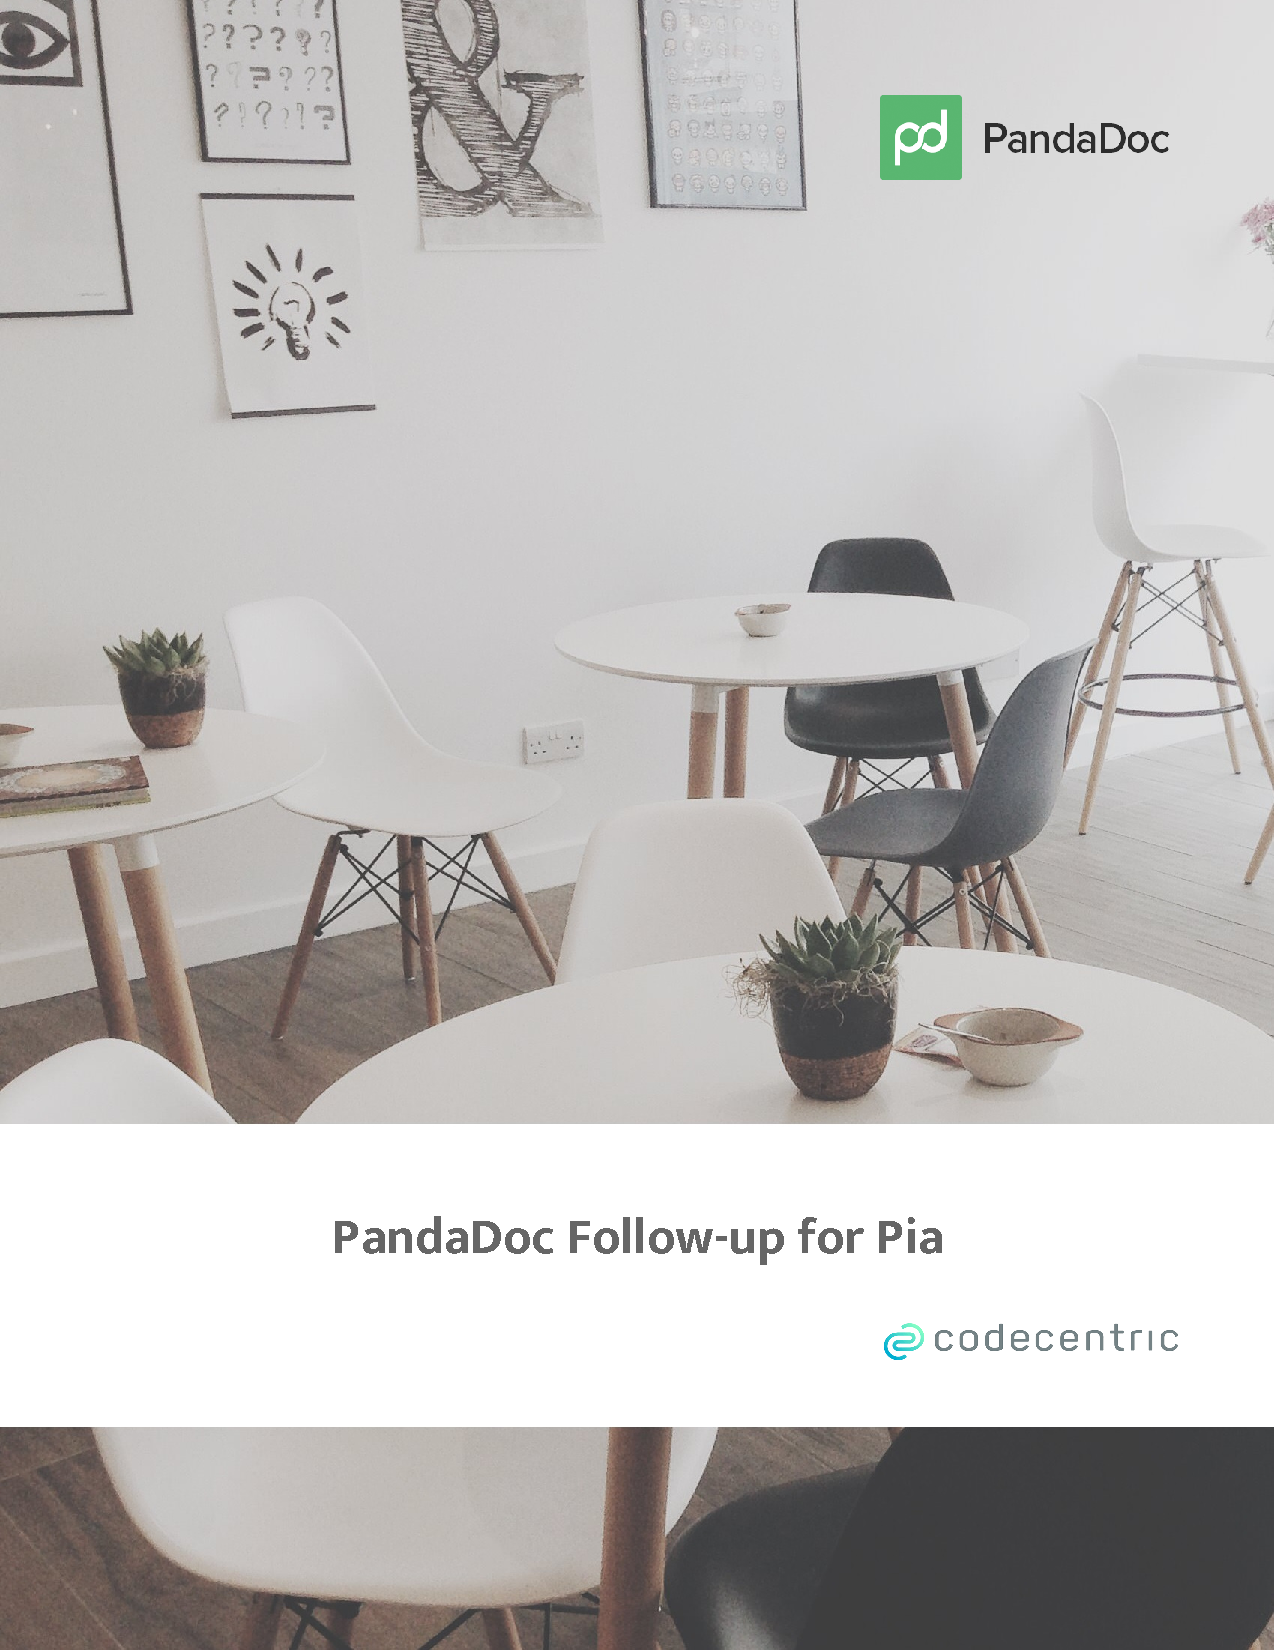
\includepdf[pages=-]{./toolResearch/docs/PandaDocFollow-upforPia.pdf}

\section{Price Information DocuSign} \label{tool:sec:docusignPrice}

\includepdf[pages=-]{./toolResearch/docs/DocuSign.pdf}

\section{Price Information HelloSign} \label{tool:sec:hellosignPrice}
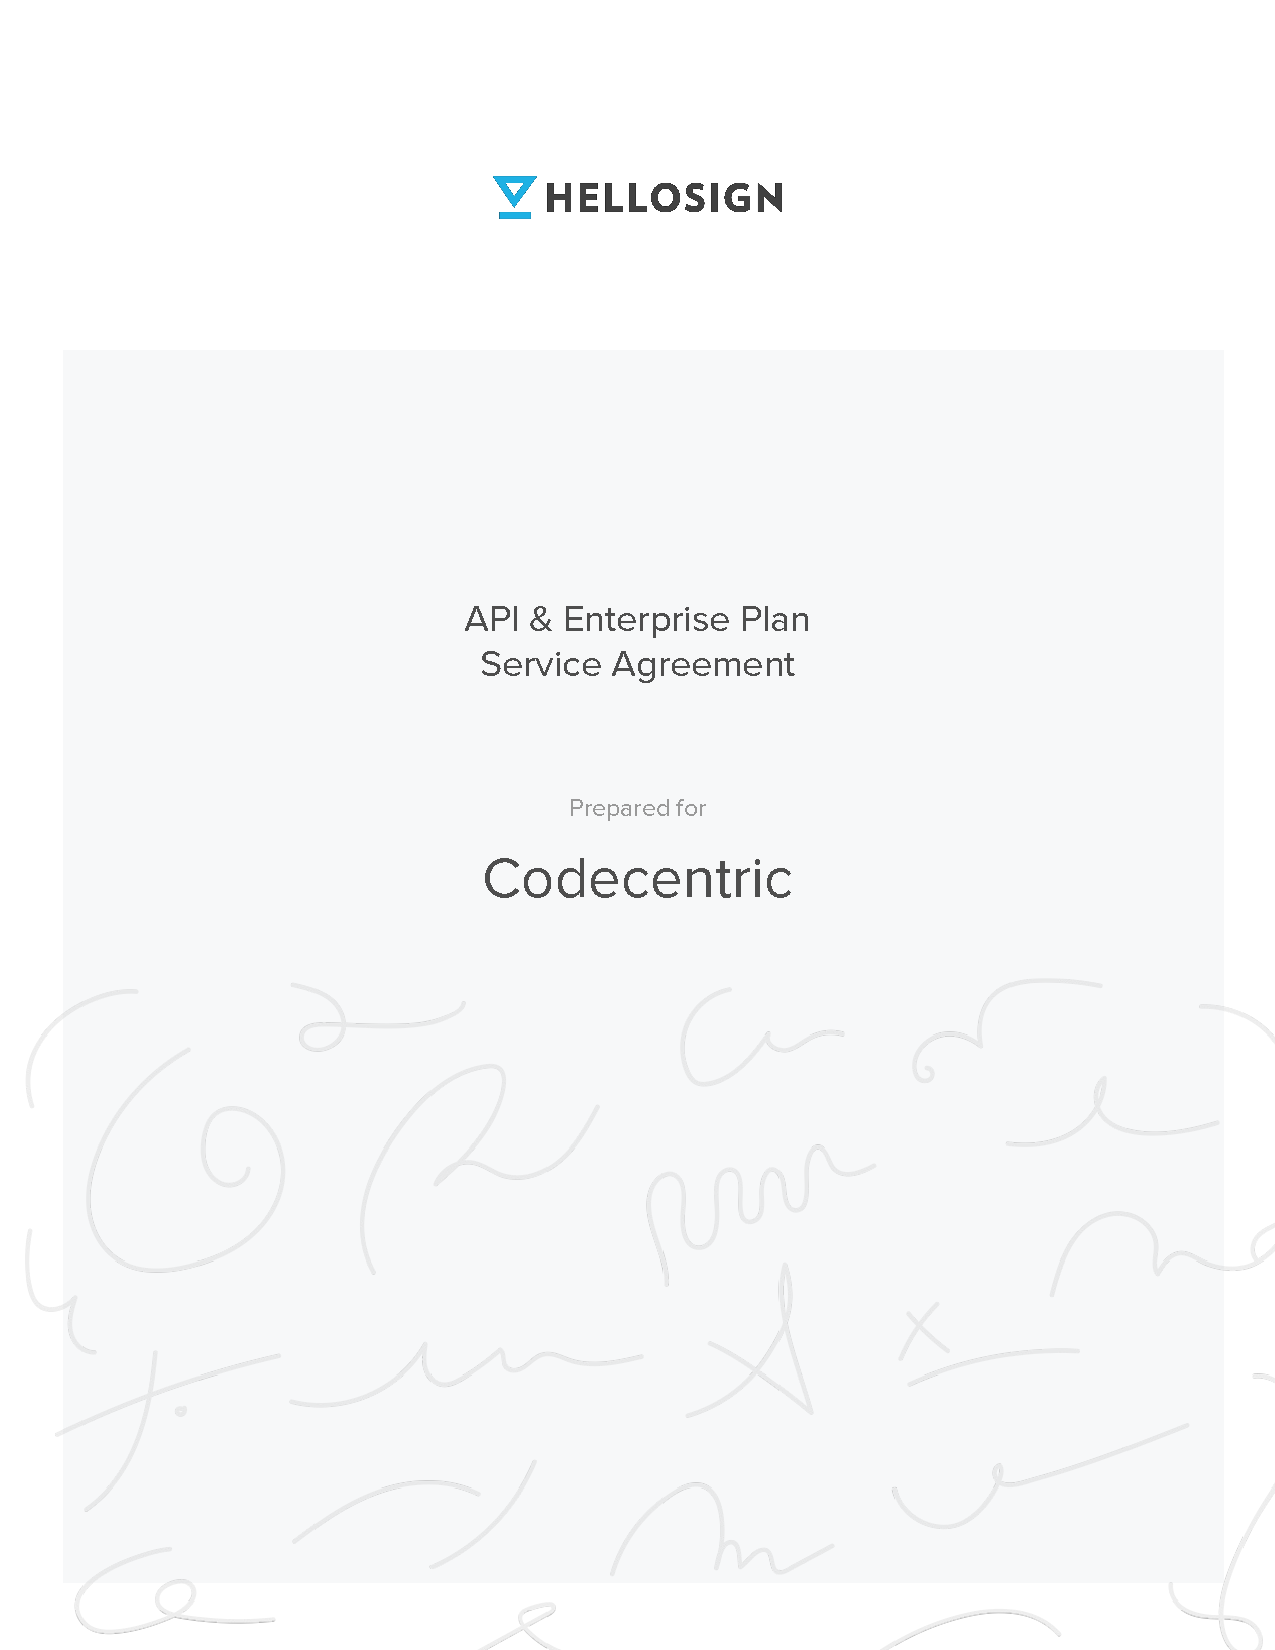
\includepdf[pages=-]{./toolResearch/docs/Codecentric.pdf}

\section{Price Information eSign Live} \label{tool:sec:esignlivePrice}
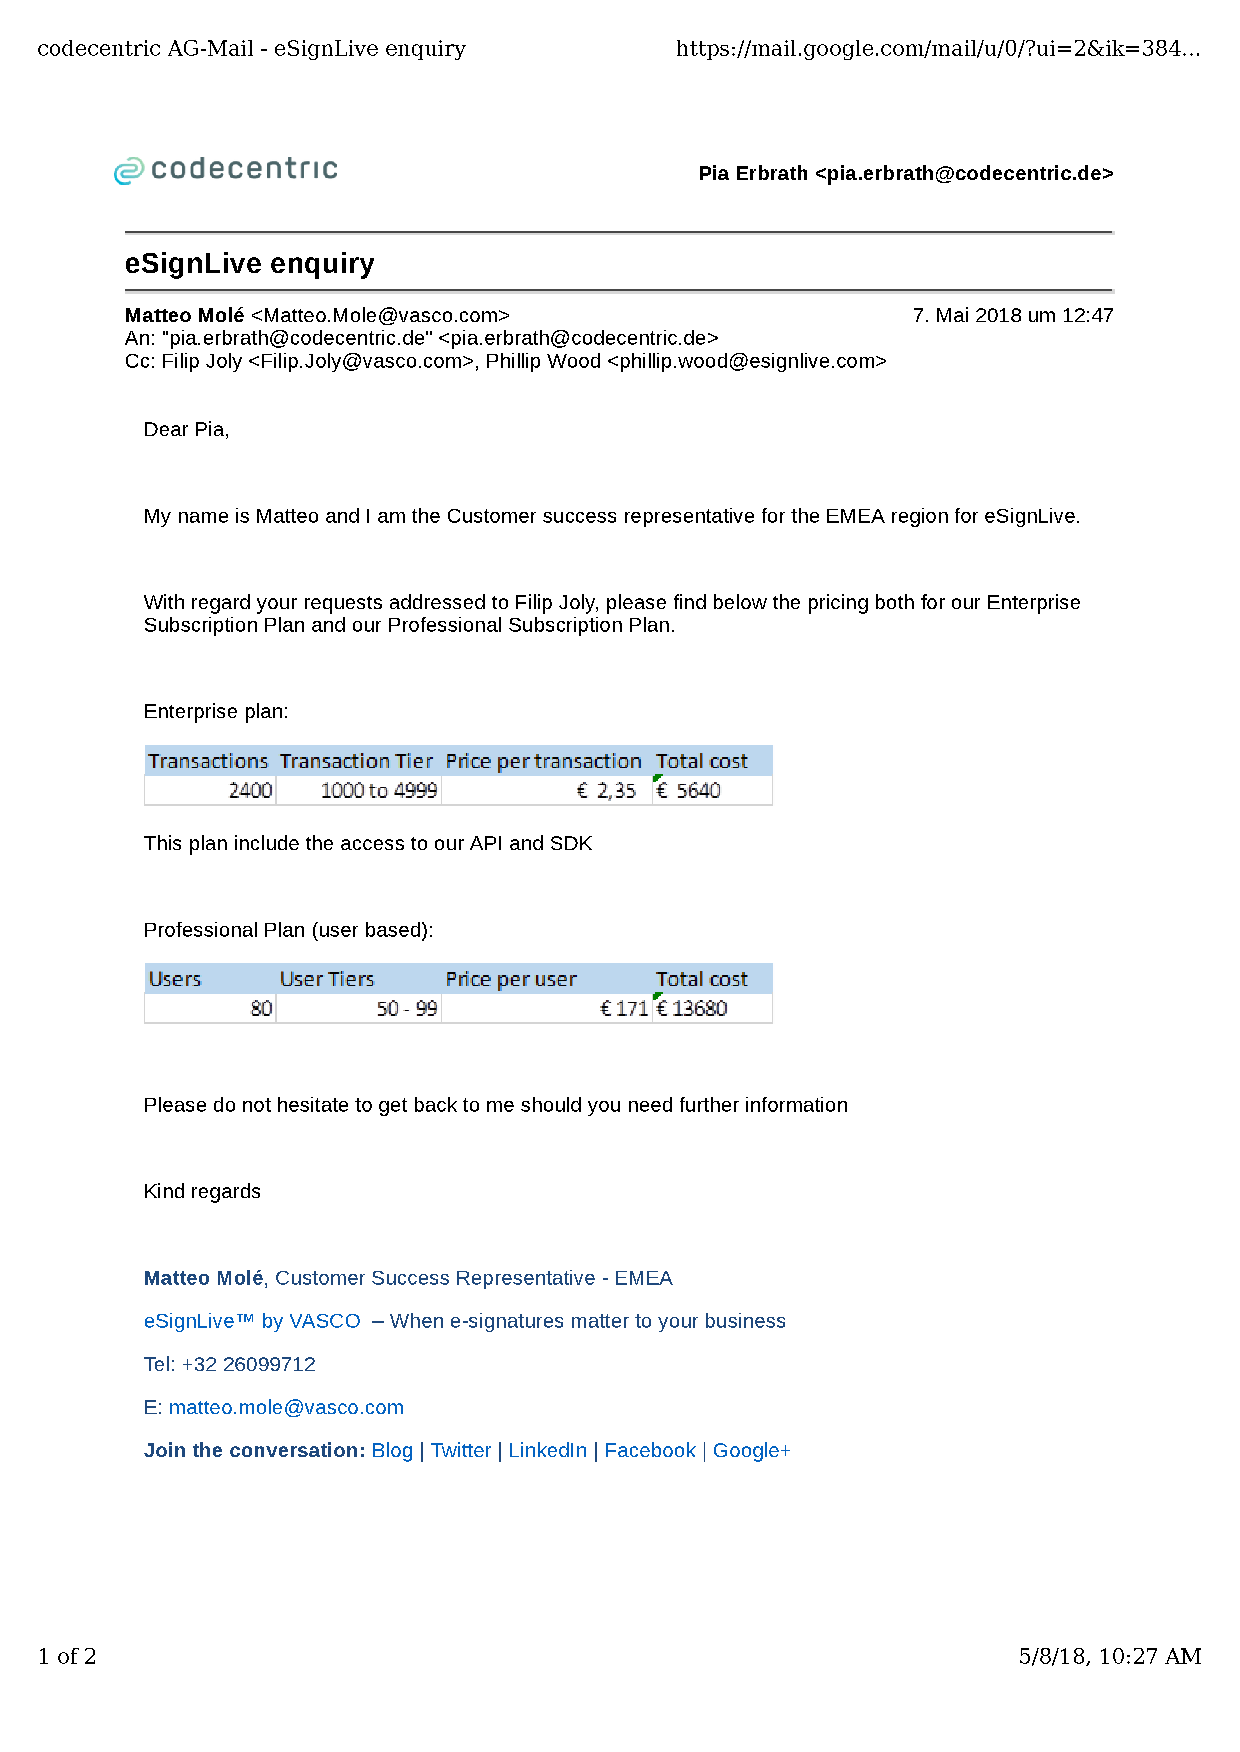
\includepdf[pages=-]{./toolResearch/docs/esignlivePrice.pdf}

\section{Price Information eSignAnyWhere} \label{tool:sec:esignanyPrice}
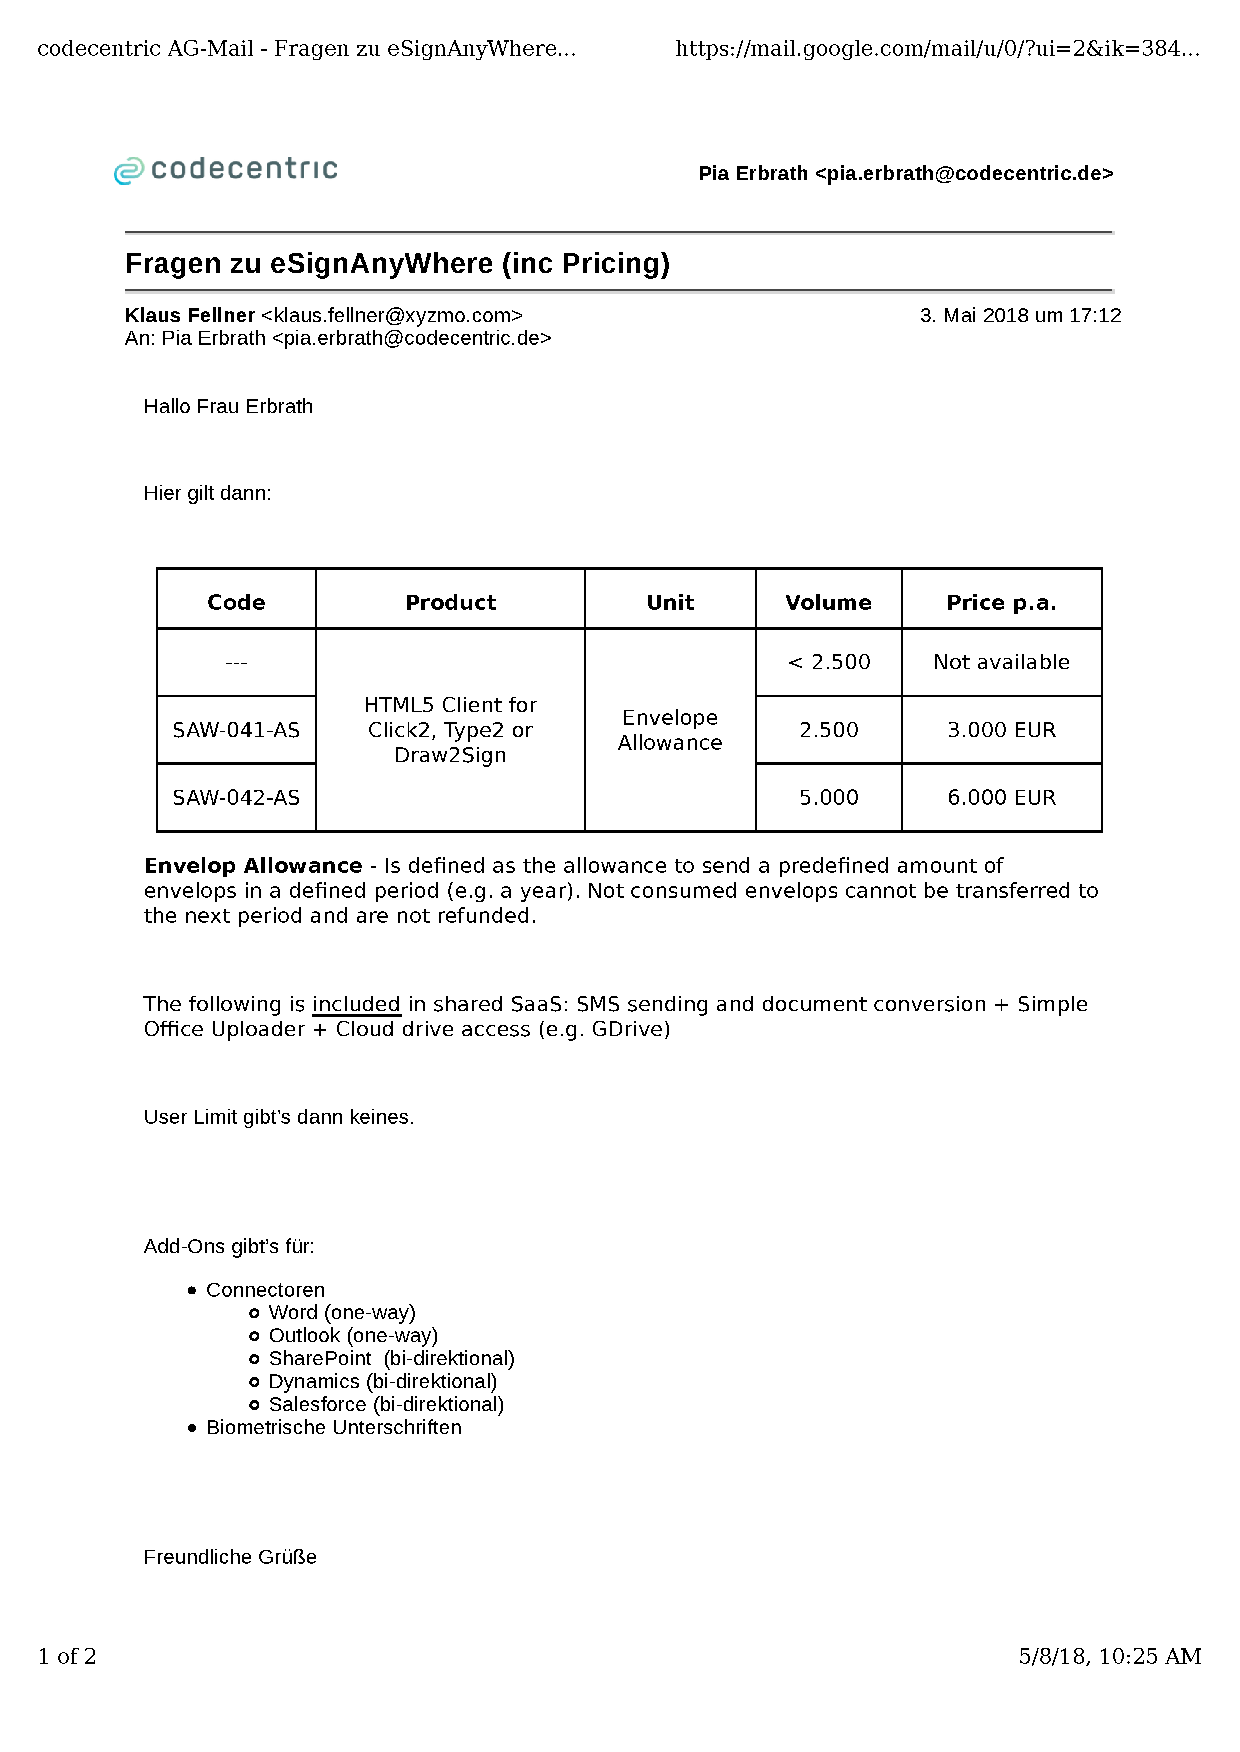
\includepdf[pages=-]{./toolResearch/docs/esignanyPrice.pdf}
	
	\chapter{Mathematical Code Representation Rule Set Request}
	\label{mathCode}
	\begin{minipage}{\textwidth}
	Existing datasets:
	\begin{itemize}
		\item $ A = set of positions at the company $
		\item $ B = set of document types at the company$
		\item $ C = \{(c_1, c_2) | c_1,c_2 \in \!R_0^+, c_1 < c_2 \}$ // set of different value ranges for documents
		\item $ D = \{(a_1, ... , a_n) | a_i \in A \}$ // set of different signing groups
		\item $ E = \{ (b, (c_1,c_2), (d_1, ... , d_n)) | b \in B, (c_1,c_2) \in C, (d_1, ..., d_n) \in D \}$ // set with signing rules containing document specification, value range specification and signing group
	\end{itemize}
	
	Function:
	\begin{algorithmic}
		\Function{f}{x,y,z} with the following conditions: $ x \in B \land z \in A \land y \in \!R_0^+$
		
		\If {$ \exists b \in B, b = x \land \exists a \in A, a = z $}
			%\State $ docs \gets \forall (x, (c_1, c_2), (d_1, ... , d_n)) \in E $
			\State $ docs = \{ (c_1,c_2) | (b, (c_1, c_2), (d_1, ... , d_n)) \in E, b = x \}$
			\State $i,j$
			\ForAll{$ (c_1, c_2) \in docs $}
				\If{$ c_1 \leq y \leq c_2 $}
					\State $ i \gets c_1$
					\State $ j \gets c_2$									
				\EndIf
			\EndFor
			
			%\State $ groups \gets \forall (x, (i,j), (d_1, ... , d_n) \in docs $
			\State $ groups = \{ (d_1, ... , d_n) | (b, (c_1, c_2), (d_1, ... , d_n)) \in E, b = x, c_1 = i, c_2 = j \}$
			\State $ inGroup[|groups|]$
			\ForAll{$ (d_1, ... , d_n) \in groups $}
				\If{$ y \in (d_1, ... , d_n) $}
					\State $inGroup [|(d_1, ... , d_n)|] = (d_1, ... , d_n)$
				\EndIf
			\EndFor
			\If{$|inGroups| > 0 $}
				\For{$k \gets 0, |inGroups|$}
					\If{$inGroups[k] \notin \emptyset$}
						\State \Return $inGroups[k]$
					\EndIf
				\EndFor
			\Else
				\State \Return error: no group for position and value found
			\EndIf			
		\Else
			\State \Return error: position/document type does not exists
		\EndIf
		
		\EndFunction
	\end{algorithmic}
\end{minipage}
	
	\chapter{Definition of Done}
	\label{definitionOfDone}
	\begin{itemize}
	\item The requested functionalities are all implemented
	
	\item Code and Build Management
	\begin{enumerate}
		\item Everything compiles without errors and warnings
		\item Sources are under version control in Gitlab
		\item Build dependencies are explicitly managed with Maven
	\end{enumerate}

	\item Testing
	\begin{enumerate}
		\item Unit tests exist and are green
		\item Integration tests exist and are green
		\item Application has been manually tested
		\item Browser independent testing is done for Chrome and Firefox
	\end{enumerate}

	\item Quality
	\begin{enumerate}
		\item Code is refactored for maintainability
		\item Clean Code (\url{https://de.wikipedia.org/wiki/Clean_Code})
		\item SOLID (\url{https://en.wikipedia.org/wiki/SOLID})
		\item Code documentation (class, method, diagrams)
		\item Documentation exists and is up-to-date
		\item User documentation
		\item Admin documentation
		\item Developer documentation
		\item Code satisfy the coding guidelines based on the following link:  \url{https://google.github.io/styleguide/javaguide.html}
	\end{enumerate}	
\end{itemize}
	
	\chapter{Product Backlog}
	\label{productBacklog}
	\begin{landscape}
	\begin{figure}
		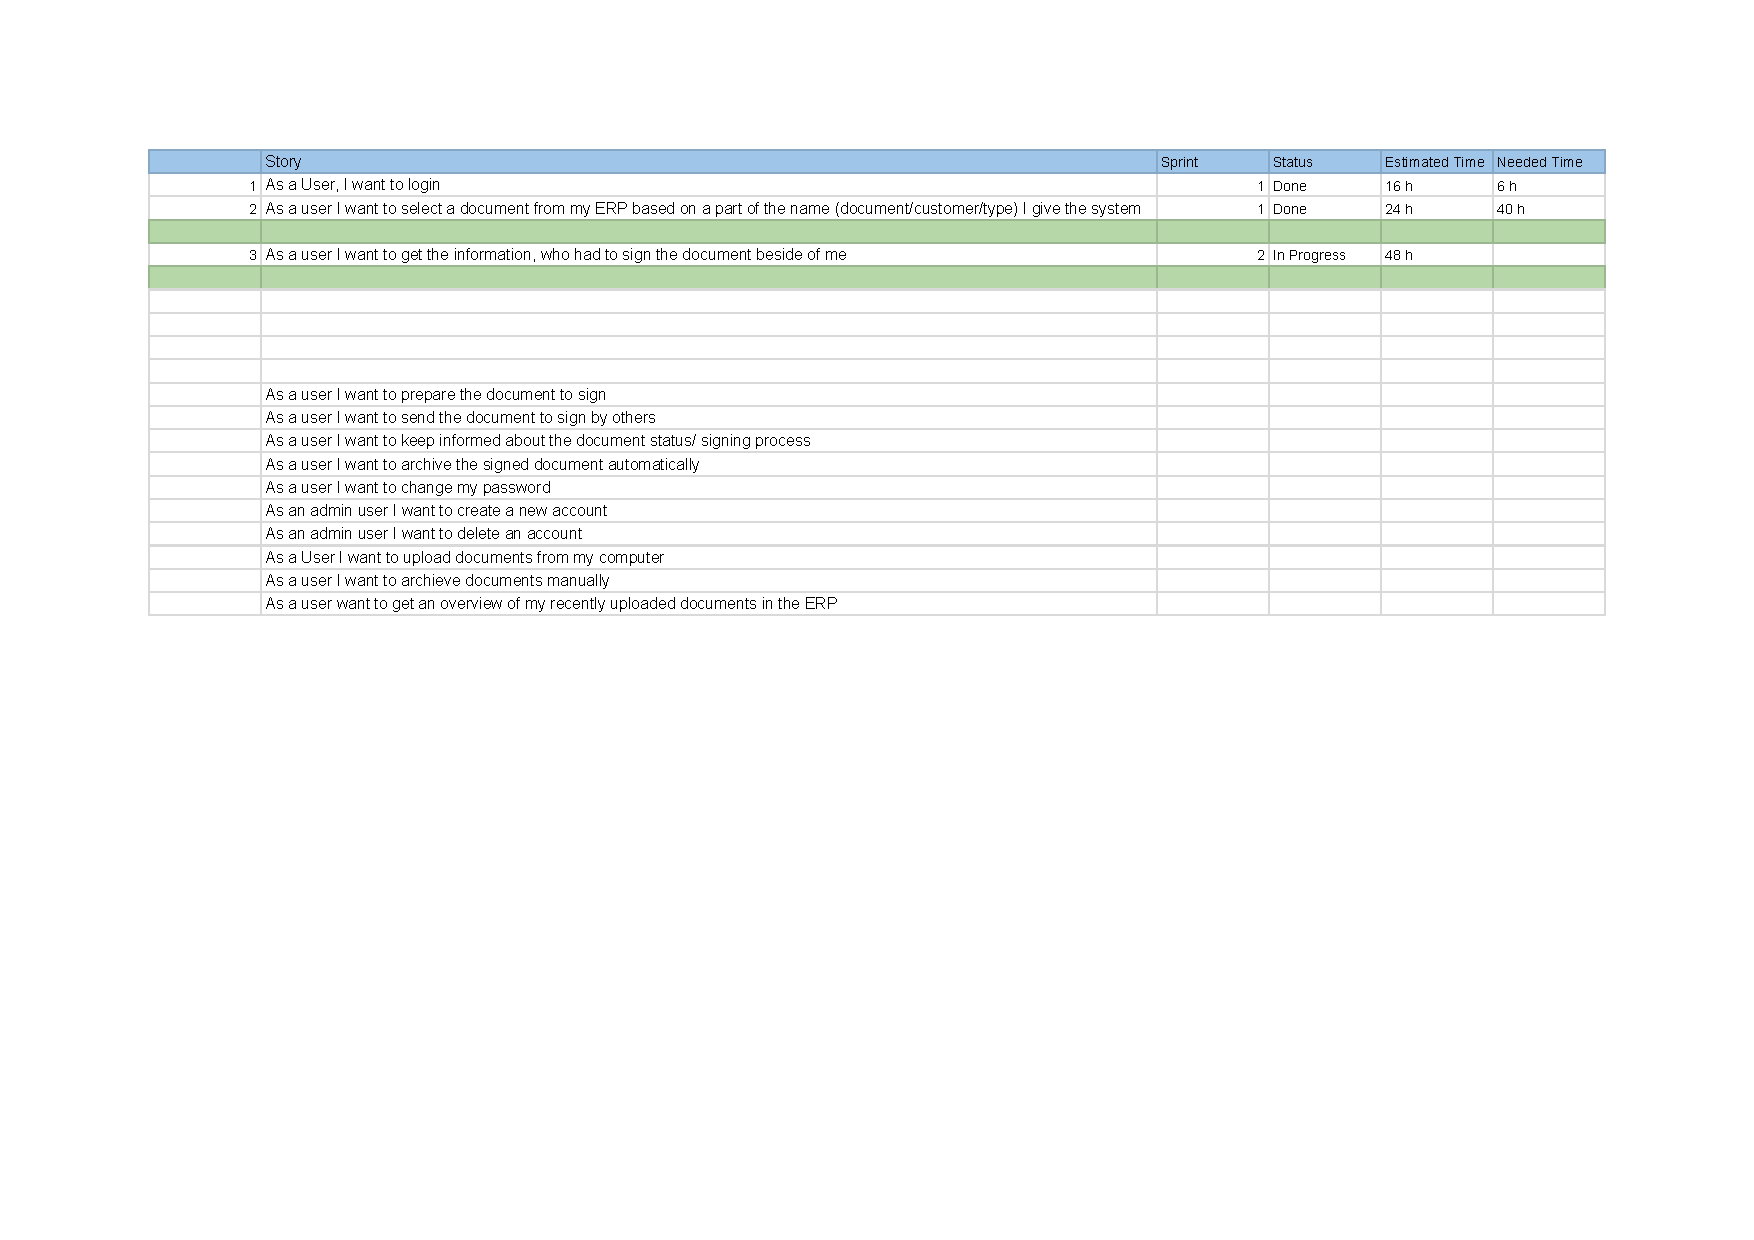
\includepdf[pages=1,landscape=true]{./appendix/productBacklog/ProductBacklog-UserStories.pdf}
		\caption{Product backlog with all User Stories and Sprint Backlogs}
	\end{figure}
\end{landscape}


	
	\chapter{User Management Server File}
	\label{ap:userManagement}
	\begin{lstlisting}

dn: ou=codecentric,dc=codecentric,dc=com
objectclass: top
objectclass: organizationalUnit
ou: codecentric

dn: ou=groups,ou=codecentric,dc=codecentric,dc=com
objectclass: top
objectclass: organizationalUnit
ou: groups

dn: ou=people,ou=codecentric,dc=codecentric,dc=com
objectclass: top
objectclass: organizationalUnit
ou: people

dn: uid=john.doe,ou=people,ou=codecentric,dc=codecentric,dc=com
objectclass: top
objectclass: person
objectclass: organizationalPerson
objectclass: inetOrgPerson
cn: John Doe
sn: Doe
mail: johnathan.doe@web.de
uid: john.doe
userPassword: john.doe

dn: cn=employee,ou=groups,ou=codecentric,dc=codecentric,dc=com
objectclass: top
objectclass: groupOfNames
cn: employee
member: uid=john.doe,ou=people,ou=codecentric,dc=codecentric,dc=com

\end{lstlisting}
	
	\chapter{Classdiagrams Mocked Components}
	\section{User Management Mock}
\begin{figure}[h!]
	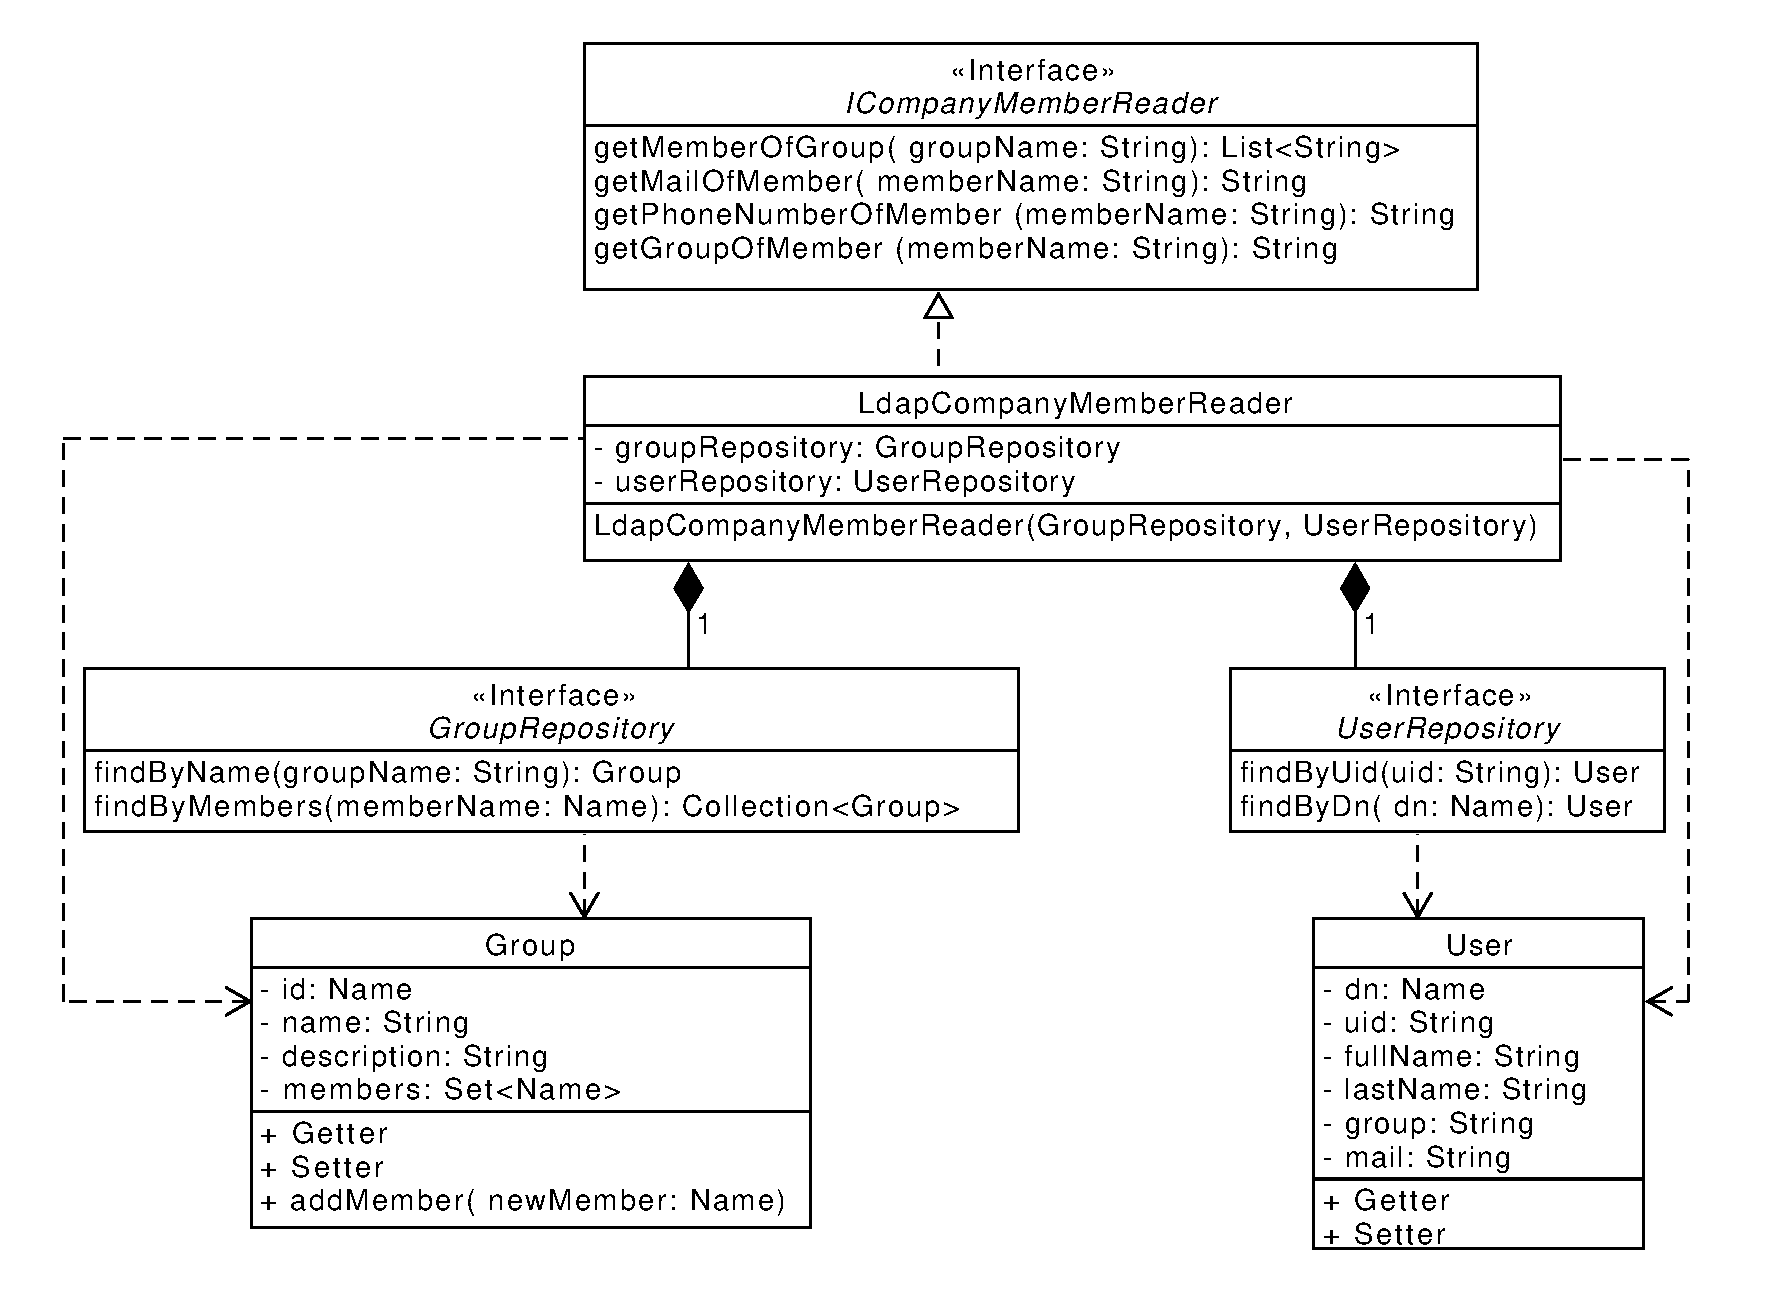
\includegraphics[width=\textwidth]{./implementation/images/ldapMock.pdf}
	\centering
	\caption{Classdiagram LDAP Reader}
	\label{fig:ldapMock}
\end{figure}

\section{Rule Set Mock}
\begin{landscape}
	\begin{figure}[h!]
		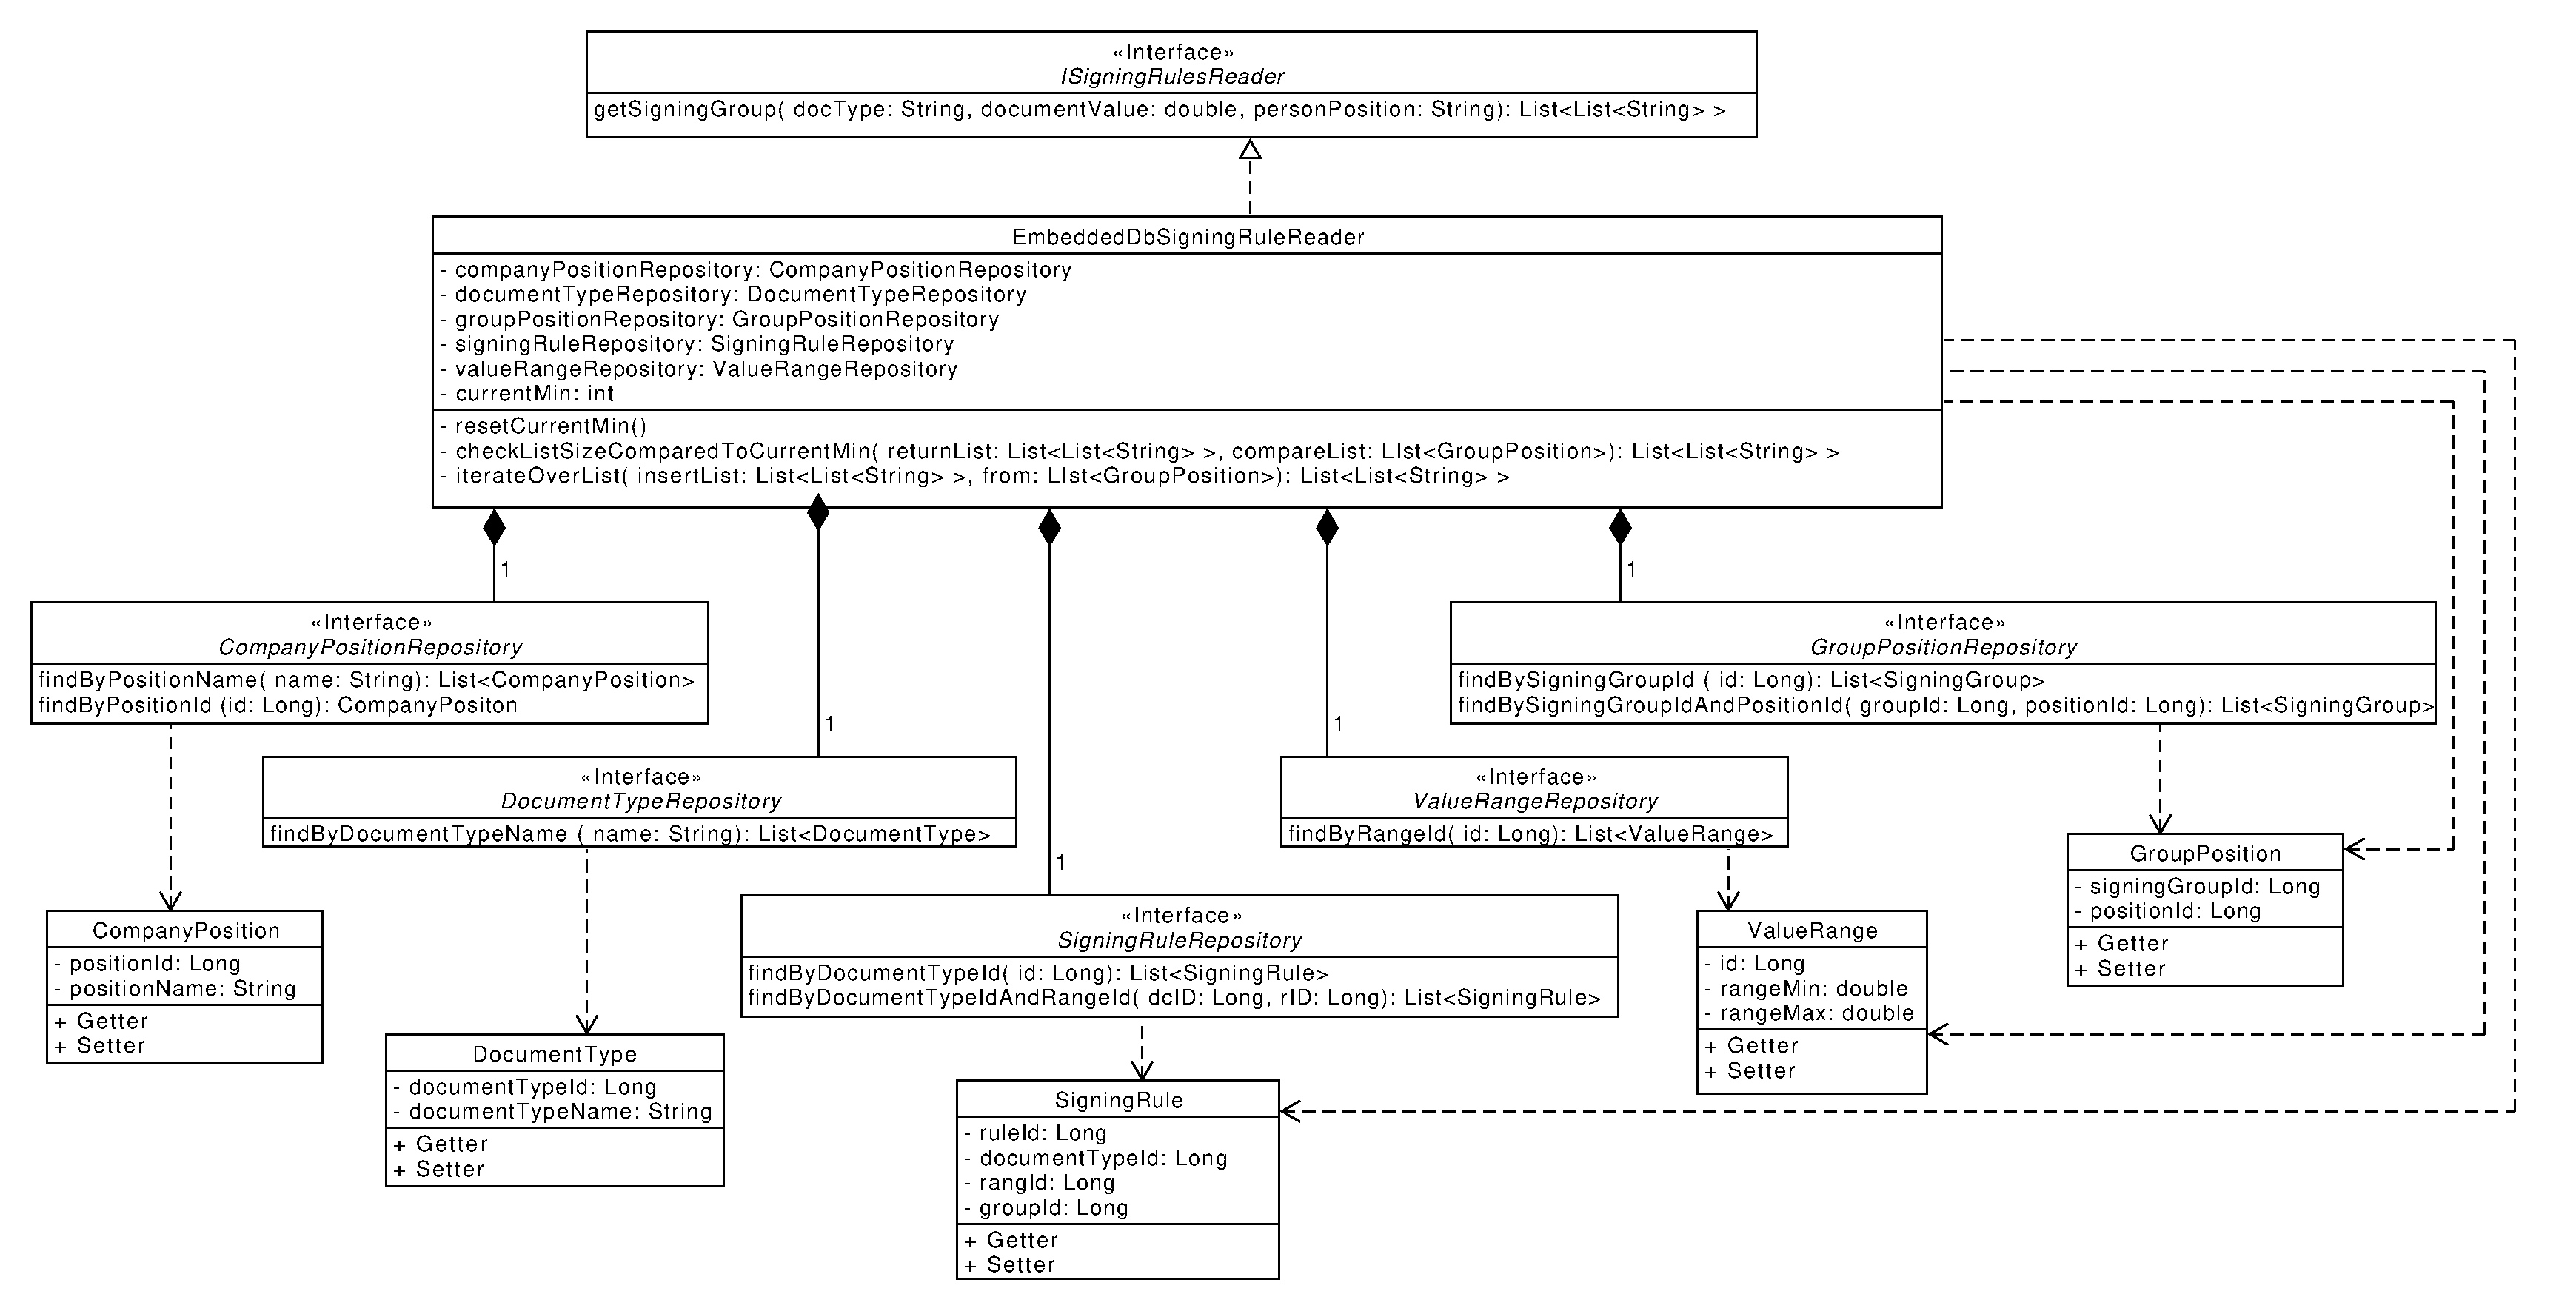
\includegraphics[width=1.48\textwidth]{./implementation/images/dbMock.pdf}.
		\centering
		\caption{Classdiagram Rule Set Reader}
		\label{fig:dbMock}
	\end{figure}
\end{landscape}
	
\end{document}